%=========================================================================
%Jakub Bartecek (xbarte09)
%Date: 2013 - 2014
%Encoding: UTF-8
%set syntax=tex
%\listoffigures

\chapter{Úvod}
    Tato diplomová práce se zabývá vylepšením serveru Jenkins CI, který je v~praxi využíván pro potřeby průběžného testování softwaru
    a~jeho kontinuální integraci. Vylepšení se týká především webového serveru a~\emph{servlet} kontejneru, který je v~Jenkins CI integrován. 
    V~současném stavu tyto funkce vykonává kombinace serverů Winstone a~Jetty. 
    
    Server Winstone je již neudržovaný a~zastaralý nástroj a~z~tohoto důvodu
    byl z~velké části nahrazen serverem Jetty, který potřebnou funkcionalitu poskytuje. Server Jetty je poměrně komplexní projekt a~nabízí
    mnoho funkcionality, ale na druhou stranu jeho rozsah nedovoluje poskytovat maximální rychlost.
    
    V~současné době vznikl nový webový server Undertow, který si klade za cíl být co nejjednodušší a~nejrychlejší a~mohl by být přínosný
    a~vhodný pro Jenkins CI. Jelikož tento server je nový a~je sponzorován firmou Red Hat, tak lze předpokládat, že jeho vývoj
    bude nadále pokračovat a~nebude zastarávat.

    Cílem této práce je nahradit server Jetty a~případně i~server Winstone pomocí serveru Undertow 
    a~integrovat jej se serverem Jenkins CI. Při integraci je kladen důraz na snahu
    zachovat zpětnou kompatibilitu s~původním řešením. 

    V~rámci této diplomové práce jsou nejprve rozebírány potřebné informace týkající se jednotlivých nástrojů a~plánované integrace.
    Následně je detailně analyzována architektura Jenkins CI a~způsob jeho integrace se servery Winstone a~Jetty. V~navazující části
    je diskutována varianta nahrazení pouze serveru Jetty a~varianta nahrazení serveru Jetty i~Winstone pomocí serveru Undertow. 
    Z~provedené analýzy byla zvolena jedna varianta, která byla vybrána pro následnou integraci. 

    %TODO popis implementace a performance testování

    



%%%%%%%%%%%%%%%%%%%%%%%%%%%%%%%%%%%%%%%%%%%%%%%%%%%%%%%%%%%%%%%%%%%%%%%%%%%%%%%%%%%%%%%%%%%%%%%
%%%%%%%%%%%%%%%%%%%%%%%%%%%%%%%%%%%%%%%%%%%%%%%%%%%%%%%%%%%%%%%%%%%%%%%%%%%%%%%%%%%%%%%%%%%%%%%
\chapter{Jenkins CI a~související nástroje}
    Tato kapitola se zaměřuje na teoretické základy práce, které je nutné nebo vhodné znát pro pochopení zpracovávané problematiky.
    Je zde detailněji popsán systém Jenkins CI (kapitola~\ref{jenkins}) ke kterému se tato práce přímo váže. S~ním je spojeno seznámení
    se servery Winstone (kapitola \ref{winstone}) a~Jetty (kapitola \ref{jetty}), jejichž kombinace je současně v~Jenkins CI integrována.
    Po popisu těchto serverů je rozebírán průběh jejich využití v~servlet kontejneru Jenkins CI a~průběh jeho vývoje (kapitola \ref{vyvojWinstone}). 
    V~kapitole \ref{servletWebserver} jsou vysvětleny často zde používané pojmy \emph{servlet kontejner} a~webový server.

    Větší důraz je dále věnován serveru Undertow (kapitola \ref{undertow}), který byl vybrán jako nový webový server pro Jenkins CI. V~tomto případě je provedena hlubší studie
    tohoto nástroje, aby na jejím základě bylo možné pochopit a~provést samotnou integraci s~Jenkins CI, která je jádrem této práce. 
    %Pro poskytnutí ucelených informací
    %je menší prostor také vymezen pro nástroj Maven (kapitola \ref{maven}), který se používá k řízení překladu serveru Jenkins CI, a je v této práci několikrát zmiňován. 

    Uvedené informace mají spíše informativní charakter, aby poskytly ucelený úvod do zkoumané problematiky. Jsou zaměřeny především na informace týkající se samotné
    integrace. Pro případné získání detailnějších informací jsou uvedeny patřičné zdroje, kde je lze nalézt.

    %%%%%%%%%%%%%%%%%%%%%%%%%%%%%%%%%%%%%%%%%%%%%%%%%%%%%%%%%%%%%%%%%%%%%%%%%%%%%%%%%%%%%%%%%%%%%%%
    \section {Jenkins CI} \label{jenkins}
        Jenkins CI je komunitní open source nástroj pro kontinuální integraci softwaru, který je vyvíjen pod svobodnou licencí
        MIT\footnote{Licence MIT: \texttt{http://opensource.org/licenses/MIT}} \cite{jenkinsGovernance}.
        Je velmi populární a~využíván malými i~velkými firmami jako je například firma Red Hat, kde tento program běží na stovkách serverů.
        Původní název tohoto projektu je Hudson\footnote{Webové stránky projektu Hudson: \texttt{http://hudson-ci.org/}}. 
        Když se jeho vývoje ujala firma Oracle, tak se projekt
        rozštěpil a~vznikla jeho komunitní verze, kterou je projekt Jenkins CI. Přesto se v~některých částech tohoto projektu 
        stále objevuje název Hudson, ale jedná se pouze pozůstatek z~původního projektu.

        Zkratka CI je z~anglického spojení \emph{continuous integration}, což lze do češtiny přeložit jako kontinuální nebo průběžná 
        integrace. Krátké seznámení s~touto metodologií je v~následující kapitole.

        Informace v~této kapitole byly čerpány především  z~knihy \cite{jenkinsBook}, kde lze nalézt další informace o~serveru Jenkins CI,
        a~také z~webové stránky projektu \cite{jenkinsWeb}.

        \subsection{Kontinuální integrace a~využití Jenkins CI}
            V~minulosti byla integrace programu do výsledného produktu velmi náročným procesem a~často ztraceným časem.
            S~vydáním každé verze programu se musel postup probíhající před vydáním produktu opakovat a~pro tým vývojářů
            to prakticky znamenalo zdržení. Pokud se v~tomto procesu odhalil nějaký problém (což bylo běžné),
            tak jeho řešení bylo z~důvodu nedostatku času a~jeho pozdního objevení mnohem problematičtější
            než kdyby byl tento problém odhalen dříve.

            Kontinuální integrace je moderní přístup k~vývoji softwaru, který mění způsob přemýšlení nad celým procesem vývoje
            a~snaží se předcházet problémům popsaným výše a~především ušetřit čas. V~tomto přístupu je využíván nějaký
            kvalitní nástroj, který automatizovaně provádí specifikované kroky, které provázejí integraci softwaru a~jeho vydání.

            Jedním z~nástrojů poskytujících podporu pro kontinuální integraci při vývoji softwaru je 
            server Jenkins CI. 
            
            \medskip \noindent Základními možnostmi, které umožňuje Jenkins CI nakonfigurovat, jsou:
            
            \begin{itemize}
                \item Spouštění integračních a~jednotkových testů v~přesně definovaném čase (např. v~noci, kdy jsou servery méně vytížené)
                \item Spuštění integračních a~jednotkových testů při změně ve verzovacím systému. Jenkins CI dokáže zaznamenat změnu v~repozitáři,
                    stáhnout si změny a~spustit testování
                \item Shromažďování a~vyhodnocování metrik vývoje softwaru
                \item Spuštění akceptačních testů
                \item Informování e-mailem o~testech, které skončily chybou
                \item Automatické nahrání nové verze produktu na server
            \end{itemize} 

            Uživatelé mohou kdykoliv přidat využití libovolné funkcionality systému a~neopakovat stále stejné kroky. 
            

        \subsection{Způsoby použití aplikace}
            Celý program je napsán v~jazyce Java a~je tedy plně přenositelný mezi platformami. Architektura je navržena tak, aby byla 
            lehce rozšiřitelná pomocí tzv. \emph{pluginů}, kterých je pro něj vytvořené velké množství. 
            
            Jenkins CI je určen pro běh na serveru a~je dostupný přes webové rozhraní (ale může být samozřejmě spuštěn
            na libovolném osobním počítači). Komunikuje pomocí protokolu \emph{HTTP}, 
            který je založen na modelu \emph{požadavek-odpověď} (angl. \emph{request-response}). Jelikož tento způsob komunikace
            je velmi běžný, tak není v~programu přímo implementován, ale využívá k~němu externí nástroje. 
            Dalším nástrojem, který pro svou činnost Jenkins potřebuje, je servlet kontejner ve kterém samotná 
            aplikace poběží.
            Tento pojem je blíže objasněn v~kapitole \ref{servletWebserver}.

            \medskip \noindent
            Existují dvě možnosti jak spustit server Jenkins CI:

            \begin{enumerate}
                \item{Může běžet na libovolném \emph{Java EE} aplikačním serveru \cite{jenkinsServers} jako jsou například servery 
                JBoss\footnote{Více informací o~serveru viz \texttt{http://www.jboss.org/jbossas/}} 
                anebo Glasfish\footnote{Více informací o~serveru viz \texttt{http://www.oracle.com/technetwork/middleware/glassfish/}}}.
                Jenkins CI se standardně nasadí na server (dle zvyklostí konkrétního serveru)
                a~poté je s~ním možné pracovat. V~tomto případě veškerou nízkoúrovňovou komunikaci pomocí síťových protokolů 
                i~práci servlet kontejneru zajišťuje aplikační server.
                
                \item{Pokud nechceme nebo nemůžeme spouštět Jenkins CI na aplikačním serveru, tak jej lze spustit přímo
                    z~vytvořeného \texttt{.war} archivu (překladem se zabývá kapitola \ref{jenkinsUsage}). V~tomto případě
                    se o~práci servlet kontejneru i~webového serveru komunikujícího jedním ze standardních síťových protokolů stará 
                    kombinace nástrojů Winstone a~Jetty, které jsou přímo integrovány do serveru Jenkins CI. 
                    
                    Nahrazení těchto dvou nástrojů (nebo pouze serveru Jetty) a~zajištění vykonávání této činnosti je hlavním cílem této práce.
                    Záměrem je tedy nahradit server Jetty a~případně i~server Winstone pomocí zvoleného nového serveru Undertow.
                    Studie těchto nástrojů a~jejich rozbor je předmětem následujícíh kapitol.}
            \end{enumerate}

            Pro tuto práci je důležitý druhý způsob používání Jenkins CI a~proto další informace se budou přímo vázat k~němu.

         \subsection{Architektura serveru}   \label{secJenkinsArchitektura}
            Architektura systému Jenkins CI je poměrně komplikovaná a~pro tuto práci není nutné ji detailně celou znát.
            Bude popsána na vysoké úrovni abstrakce a~zaměří se pouze na komponenty, které se přímo týkají této práce
            a~budou dále v~textu odkazovány nebo blíže rozebírány. Přehled architektury je na obrázku~\ref{imgJenkinsArchitecture}.
       
            \begin{figure}[ht]
                \begin{center}
                    \scalebox{0.65}{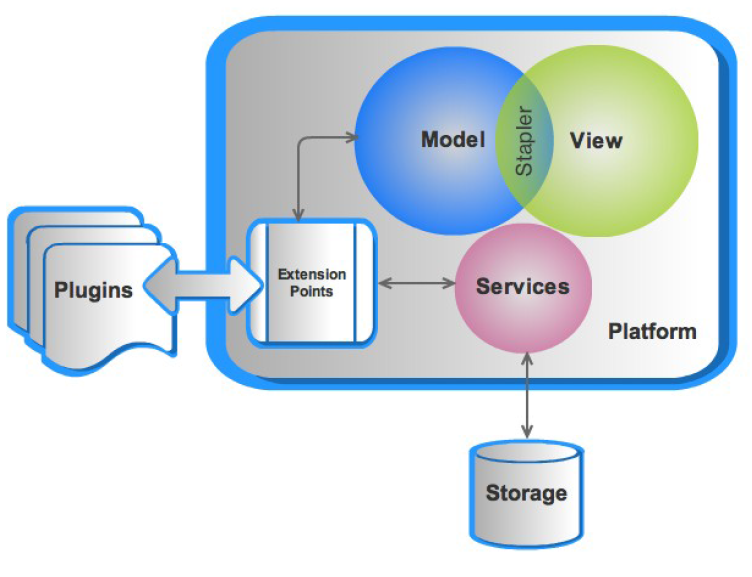
\includegraphics{img/jenkinsArchitecture.png}}
                    \caption{Přehled architektury serveru Jenkins CI \cite{architectureOverview}}
                    \label{imgJenkinsArchitecture}
                \end{center}
            \end{figure}     

            Základem architektury je část \emph{Model}, což jsou objekty, které obsahují stav
            a~data aplikace. Každý model je přímo navázán na konkrétní URL adresu s~tím, že kořenový
            model (dostupný pod URL \uv{/}) je pevně daná instance s~názvem \texttt{Hudson}.
            Data z~objektů modelu jsou následně zobrazovány ve webovém rozhraní aplikace.
            Pro toto zobrazování je využita techonologie Jelly.

            Velmi podstatnou součástí aplikace je prvek \emph{Stapler}. Tento objekt
            provádí konkrétní propojování požadavků dle zadané URL s~patřičnými objekty
            z~modelu a~spouštění vykonávání jejich metod. Stapler je
            jediným servletem, který je v~aplikaci Jenkins CI zaveden do
            servlet kontejneru při spuštění aplikace (pojmy servlet a~servlet kontejner 
            jsou vysvětleny v~kapitole \ref{servletKontejner}).
            Povědomí o~jeho
            činnosti je potřebné, protože s~ním bude v~této práci dále pracováno.
            Průběh vybírání patřičných metod pomocí této komponenty je přesně
            definován a~lze jej najít v~uživatelské příručce\footnote{
                Způsob zpracovávání požadavků komponentou Stapler:
                \texttt{http://stapler.kohsuke.org/reference.html}}, 
                ale není nutné jej zde rozebírat.

            Architektura serveru je přizpůsobena tak, aby byla snadno rozšiřitelná
            pomocí rozšiřujících modulů (angl. \emph{plugins}). Popis technologie Jelly
            i~tvorba rozšiřujících modulů je nad rámec této práce a~lze tyto informace
            najít v~odkazované literatuře.
        
            Informace v~této kapitole byly čerpány z~tohoto dokumentu \cite{architectureOverview}
            a~z~webových stránek projektu Stapler \cite{staplerWeb}.

        \subsection{Základy práce s~Jenkins CI} \label{jenkinsUsage}
            Pro přeložení a~spuštění aplikace je potřeba pracovat z~příkazové řádky nebo provést instalaci nějakým dávkovým souborem (skriptem).
            Aplikaci je možné stáhnout připravenou přímo ze stránek projektu \cite{jenkinsWeb}, ale pro tuto práci je potřeba 
            pracovat s~aplikací ze zdrojových souborů. Aktuální verze aplikace je dostupná na serveru 
            GitHub\footnote{Adresa aktuální verze Jekins CI: \texttt{www.github.com/jenkinsci}}.

            Po stažení zdrojových souborů je potřeba provést překlad aplikace. Pro tento automatizovaný 
            překlad se používá nástroj Maven\footnote{Více informací o~nástroji Maven lze získat na stránce 
            \texttt{http://maven.apache.org/}},který je krátce zmíněn v~kapitole \ref{maven}. 
            
            Překlad aplikace bez spuštění jednotkových testů i~integračních testů lze provést tímto příkazem:
            \begin{verbatim}
                mvn clean install -pl war -am -DskipTests
            \end{verbatim}
            
            \medskip
            Po úspěšném překladu aplikace vznikne v~adresáři \texttt{./war/target/} archiv \texttt{jenkins.war}, 
            který obsahuje celou přeloženou webovou aplikaci včetně nástrojů na 
            kterých závisí. Z~tohoto archivu je možné aplikaci přímo spustit pomocí příkazu:

            \begin{verbatim}
                java -jar jenkins.war
            \end{verbatim}
            Chování aplikace lze upravit nastavením různých parametrů při spuštění programu, 
            které lze vypsat pomocí přidání parametru \texttt{--help}.

            Pro práci se spuštěnou instancí aplikace se používá především webové rozhraní. Standardně aplikace
            komunikuje pomocí protokolu \emph{HTTP} na portu 8080. Je tedy možné se na lokálním počítači připojit do aplikace zadáním URL adresy 
            \texttt{http://localhost:8080} do webového prohlížeče. 

            Pokud se aplikaci povede spustit, tak je již možné libovolně pracovat pouze s~prohlížeče. Detaily práce s~aplikací Jenkins CI
            lze nalézt v~této knize \cite{jenkinsBook}, ale tyto informace jsou již nad rámec této publikace.


            
       
    %%%%%%%%%%%%%%%%%%%%%%%%%%%%%%%%%%%%%%%%%%%%%%%%%%%%%%%%%%%%%%%%%%%%%%%%%%%%%%%%%%%%%%%%%%%%%%%
    \section{Webový server a~servlet kontejner} \label{servletWebserver}
        V~této kapitole jsou vysvětleny pojmy webový server a~servlet kontejner, které se 
        na mnoha místech této práce objevují. Porozumění těmto pojmům je důležité, protože bez
        jejich znalosti by následující kapitoly byly obtížněji pochopitelné.
        
        Informace zde uvedené byly čerpány z~článku \cite{webserverVsServletPage}.

        \subsection{Webový server}
            Webový server je program, který zprostředkovává komunikaci přes síť s~klienty, kteří
            se k~němu připojí a~požadují po něm nějaká data. Tato komunikace běžně probíhá pomocí protokolu \emph{HTTP}
            nebo jeho šifrované verze \emph{HTTPS},
            které jsou založeny na modelu \emph{požadavek-odpověd} (angl. \emph{request-response}).
            Model této komunikace je zachycen na obrázku \ref{imgWebserver}.
            
            Typický způsob komunikace webového serveru je, 
            že klient pomocí URL adresy specifikuje požadavek na nějaká
            data a~server mu v~odpovědi tato data pošle. Pokud by neexistoval za webovým serverem nějaký další
            program, tak by webový server vždy odpovídal na stejný požadavek stále stejnou odpovědí.

            \begin{figure}[ht]
                \begin{center}
                    \scalebox{0.63}{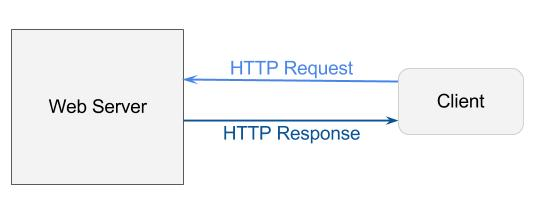
\includegraphics{img/web-server.jpg}}
                    \caption{Model komunikace webového serveru s~klientem \cite{webserverVsServletPage}}
                    \label{imgWebserver}
                \end{center}
            \end{figure}    %TODO fix obrazek je potreba prekreslit

        \subsection{Servlet kontejner} \label{servletKontejner}
            Jelikož dostávat stále stejná statická data při stejném požadavku není dostatečná funkcionalita serveru,
            tak existují způsoby jak zajistit dynamickou práci s~daty na serveru a~tudíž i~poskytovat
            měnící se odpovědi na stejný dotaz.
            Jedním ze způsobů jak této funkce docílit je využití tzv. \emph{servletů},
            které jsou navrženy pro programovací jazyk Java.

            Servlet je standardní program (konkrétně jedna třída) napsaný v~jazyce Java, 
            který implementuje rozhraní \texttt{javax.servlet}.
            Implementace tohoto rozhraní ho zavazuje k~definování několika metod, ale jinak se jedná o~běžnou
            třídu, z~které jsou při zpracovávání požadavků vytvářeny její instance. Po obdržení nějakého
            požadavku provádí zpracování vstupních dat a~následně odeslání patřičné odpovědi.

            Základní myšlenkou servlet kontejneru je umožnit dynamicky vytvářet odpovědi (často webové stránky)
            pomocí vykonávání servletů. Samotný servlet kontejner je program, který poskytuje běhové prostředí pro vykonávání servletů,
            zajišťuje jejich vytváření, vykonávání a~odstraňování. Dále se také podílí na zpracovávání příchozích požadavků, které jsou
            mu předávány od webového serveru. 

            Popsaný způsob fungování servlet kontejneru je znázorněn na obrázku \ref{imgServlet}.
            %teoreticky bych mohl dopsat něco o způsobu vyhodnocení servletu, ale to asi není podstatné
            \begin{figure}[ht]
                \begin{center}
                    \scalebox{0.75}{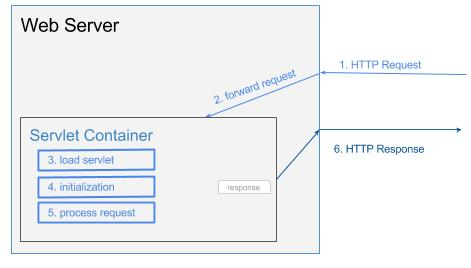
\includegraphics{img/servlet-container-life-cycle.jpg}}
                    \caption{Ukázka způsobu činnosti servlet kontejneru a~jeho spolupráce s~webovým serverem \cite{webserverVsServletPage}}
                    \label{imgServlet}
                \end{center}
            \end{figure}   %TODO fix obrazek je potreba prekreslit

        \subsection{Struktura archivu webové aplikace} \label{kapWebXml}
            Kompletní popis architektury webových aplikací v~jazyce Java by byl velmi rozsáhlý. 
            Tato kapitola se zaměřuje pouze na strukturu archivu webové aplikace \texttt{.war} pro aplikace běžící v~servlet kontejneru.
            Popis je zaměřen pouze na části, které jsou použity v~Jenkins CI a~jsou podstatné
            pro samotnou integraci serveru Undertow do Jenkins CI.

            \medskip
            Archiv \texttt{.war} je archiv zabalený metodou \emph{ZIP} a~základ jeho struktury je následující:
            
\begin{priklad} Zjednodušená struktura archivu \texttt{.war}
\begin{verbatim}
webapp.war
    |-- WEB-INF/
        |-- lib/
            |-- *.jar
        |-- classes/
            |-- *.class
        |-- web.xml
    |-- <ostatní>
\end{verbatim}
\end{priklad}


            Pro konfiguraci aplikace je nejdůležitější adresář WEB-INF a~především tyto jeho položky:

            \begin{itemize}
                \item Adresář \textbf{lib} obsahuje libovolné uživatelské knihovny, které jsou ve webové aplikaci využívány. 
                    Knihovny jsou ve standardním archivu \texttt{.jar}.
                    Servlet kontejner je zodpovědný za zavádění těchto knihoven, aby je bylo možné v~aplikaci následně využívat.

                \item Adresář \textbf{classes} obsahuje přeložené třídy, které se podílejí na činnosti aplikace. 
                    Servlet kontejner je opět zodpovědný za jejich zavedení. 

                \item Soubor \textbf{web.xml} obsahuje nejpodstatnější konfiguraci webové aplikace pro servlet kontejner.
                    Na základě tohoto souboru servlet kontejner provádí nastavené celé aplikace.
                    Jsou zde popsány veškeré \emph{servlety}, které aplikace obsahuje, pravidla pro zabezpečení aplikace,
                    \emph{filtery}, které mohou upravovat příchozí požadavky a~spousta dalších konfigurací. 
            \end{itemize}

            Kromě základních výše popsaných položek může archiv obsahovat libovolné jiné soubory pro běh aplikace jako jsou 
            HTML soubory, kaskádové styly (CSS), obrázky a~jiné. Servlet kontejner musí spravovat tyto zdroje
            a~při příchozích požadavcích je načítat. Pro odkazování těchto souborů je jako kořenový adresář považován
            samotný archiv, takže cesta k~souboru wem.xml je následující: \texttt{/WEB-INF/web.xml}.

            
         
    %%%%%%%%%%%%%%%%%%%%%%%%%%%%%%%%%%%%%%%%%%%%%%%%%%%%%%%%%%%%%%%%%%%%%%%%%%%%%%%%%%%%%%%%%%%%%%%
    \section{Nástroj Maven} \label{maven}
         %TODO zkontrolovat, jestli to dává smysl a není to moc rozvláčné
        Pro vývoj a~práci se serverem Jenkins CI v~podobě zdrojových kódů je zapotřebí nástroj Maven. 
        Jeho využití je také nutné při vytváření programu, který provede integraci serveru Undertow do Jenkins CI. 
        V~této kapitole budou o~něm poskytnuty základní informace. Pro případné bližší
        seznámení s~tímto nástrojem lze další informace získat z~webových stránek projektu \cite{mavenWeb}
        z~kterých byly čerpány informace v~této kapitole. 
        
        Maven je nástroj, který provádí činnosti spojené s~vytváření spustitelných aplikací ze zdrojových kódů 
        Je zaměřen na aplikace vytvářené v~jazyce Java. Hlavním cílem je umožnit uživatelům v~co nejkratším
        čase provádět běžné a~opakující se úkony při překladu aplikace. Především umožňuje
        provádění překladu aplikací, jejich spouštění automatizovaných jednotkových
a~integračních testů, uložení spustitelné podoby aplikace do lokálního repozitáře 
        a~případně i~nahrání vytvořené aplikace na nějaký server. 

        Je dodáván jako aplikace, která se spouští z~příkazové řádky příkazem \texttt{mvn}. Veškeré
        informace o~projektu a~definice činnosti, které má Maven provést, se specifikuje 
        v~XML souboru \texttt{pom.xml}. Mezi nejdůležitější patří definice výsledné podoby aplikace
        a~způsob jejího překladu, informace o~závislostech
        projektu na jiných knihovnách a~definice serverů z~kterých má stahovat potřebné knihovny pro svůj 
        běh i~pro běh aplikace. Po spuštění aplikace jsou tedy lokalizovány knihovny, na kterých projekt
        závisí a~uloženy v~lokálním repozitáři aniž by se o~tuto činnost uživatel musel dále starat.
        Kromě těchto praktických činností také umožňuje zveřejnit podrobnější informace o~projektu,         
        jako jsou informace o~licenci, vývojářích, adrese systému pro správu verzí, atp.

        Zmíněný lokální repozitář neslouží pouze ke stahování knihoven ze serveru, ale
        také pro ukládání lokálně vyvíjený aplikací.
        Pokud je aplikace vyvíjena lokálně a~skládá se z~více nezávislých modulů, tak je potřeba
        postupně tyto moduly přidávat do lokálního repozitáře, aby je při sestavování
        výsledného programu Maven mohl najít (na serveru je totiž nenajde). Pro přidání modulu či aplikace do 
        lokálního Maven repozitáře slouží parametr \texttt{install}.


        Na příkladu \ref{jenkinsPom} je ukázka části souboru \texttt{pom.xml}, který je vytvořen pro Jenkins~CI:
        \begin{priklad} \label{jenkinsPom} 
            Ukázka souboru \texttt{pom.xml}
\begin{verbatim}
  ...
  <repositories>
    <repository>
      <id>repo.jenkins-ci.org</id>
      <url>http://repo.jenkins-ci.org/public/</url>
  ...
  <dependency>
    <groupId>org.mockito</groupId>
    <artifactId>mockito-core</artifactId>
    <version>1.8.5</version>
  </dependency>
  ...
\end{verbatim}
        \end{priklad}

        V~části \texttt{repository} je definována cesta k~serveru, z~kterého má Maven stahovat potřebné soubory
        a~v~těle značky \texttt{dependency} je pomocí hodnot \texttt{groupId, artifactId, version} jednoznačně
        definována potřebná knihovna. Na základě těchto informací poté Maven při překladu stáhne požadovanou
        knihovnu a~při distribuci aplikace nemusí být tato knihovna k~programu přibalena. 


    %%%%%%%%%%%%%%%%%%%%%%%%%%%%%%%%%%%%%%%%%%%%%%%%%%%%%%%%%%%%%%%%%%%%%%%%%%%%%%%%%%%%%%%%%%%%%%%
    \section{Server Jetty} \label{jetty}
        Jednou z~komponent, které jsou aktuálně integrovány do serveru Jenkins CI, je webový server Jetty.
        Tento server je open source projektem vyvíjeným pod licencemi 
        Eclipse\footnote{Licence Eclipse je dostupná na adrese \texttt{http://www.eclipse.org/legal/epl-v10.html}}
        a~Apache\footnote{Licence Apache je dostupná 
        na adrese \texttt{http://www.apache.org/licenses/LICENSE-2.0.html}}. 
            Je využíván velkým množstvím nástrojů jako jsou například \emph{Eclipse IDE}\footnote{Webové stránky nástroje Eclipse IDE 
        \texttt{http://www.eclipse.org/}} nebo \emph{Google AppEngine}\footnote{Webové stránky platformy Google AppEngine
        \texttt{https://developers.google.com/appengine/}}.

        Jetty je webový server a~poskytuje funkcionalitu servlet kontejneru dle specifikace verze 3.0. 
        Je jej možné využít také jako webového klienta pro komunikaci se servery. Komunikace
        klientů i~serverů využívajících Jetty probíhá asynchronně. 
        Návrh serveru umožňuje samostatné spouštění aplikací i~jeho integraci do jiné aplikace. 

        %TODO nějaké reference na ty tachnologie, možná popsat SPDY a AJP13
        Kromě těchto základních možností obsahuje
        řadu souvisejících technologií, jako jsou SPDY, webové sokety\footnote{Oficiální stránky 
            specifikace webových soketů: \texttt{http://www.websocket.org/}}(angl. \emph{websocket}),
        JNDI, OSGi, JMX a~další. 
        Informace v~této kapitole byly čerpány z~webových stránek serveru Jetty \cite{jettyWeb}, kde lze nalézt 
        další informace o~zmíněných technologiích a~o~tomto serveru.
        
        Aktuální využití serveru Jetty v~aplikaci Jenkins CI je podrobněji rozebráno
        v~kapitole~\ref{vyvojWinstone} a~jeho srovnáním se serverem Undertow se 
        zabývá kapitola \ref{srovnani}.
        

    %%%%%%%%%%%%%%%%%%%%%%%%%%%%%%%%%%%%%%%%%%%%%%%%%%%%%%%%%%%%%%%%%%%%%%%%%%%%%%%%%%%%%%%%%%%%%%%
    \section{Servlet kontejner Winstone} \label{winstone}
        Další komponentou serveru Jenkins CI je servlet kontejner Winstone.
        Winstone je velmi jednoduchý a~poskytuje funkcionalitu
        servlet kontejneru aniž by byl zatížen velkým množstvím požadavků, které jsou ve specifikaci jazyka Java EE.
        Nikdy neposkytoval veškeré služby servlet kontejneru, které specifikace jazyka definuje. 
        V~jeho názvu je zahrnutý pouze pojem servlet kontejner, ale tato aplikace vykonává i~služby
        webového serveru odpovídající popisu v~kapitole \ref{servletWebserver}.

        Hlavními cíli projektu bylo poskytovat funkcionalitu servlet kontejneru pouze pro jednu aplikaci,
        což je opačný přístup než u~běžných aplikačních serverů jako jsou Glasfish, JBoss, aj.
        Díky jeho omezeným službám je jeho velikost velmi malá a~umožňuje jednoduchou integraci
        s~cílovou aplikací.

        Uvedené informace byly čerpány z~oficiální stránky projektu Winstone \cite{winstoneWeb}.

        \subsection{Nedostatky servlet kontejneru Winstone}
            Původní myšlenka jednoduchého servlet kontejneru byla pro projekt Jenkins CI zajímavá, ale
            kontejner Winstone má několik zásadních nedostatků kvůli kterým bylo časem jeho využití
            v~Jenkins CI problematické \cite{kohsukeTopic}. 

            Vývoj projektu Winstone již před delší dobou ustal a~tím pádem nebyla poskytována 
            žádná další podpora pro řešení a~opravování objevených nedostatků a~chyb. 
            Značné množství bezpečnostních chyb objevených v~projektu Jenkins CI bylo právě
            způsobeno tímto servlet kontejnerem.

            Zpočátku možnosti servlet kontejneru postačovaly, ale časem je potřeba, aby 
            byly přidávány nové funkcionality, které odpovídají aktuálním trendům
            a~novým specifikacím. Příkladem mohou být nové specifikace servlet kontejneru nebo
            vývoj nových technologií jako webové sokety.


    %%%%%%%%%%%%%%%%%%%%%%%%%%%%%%%%%%%%%%%%%%%%%%%%%%%%%%%%%%%%%%%%%%%%%%%%%%%%%%%%%%%%%%%%%%%%%%%
    \section{Vývoj servlet kontejneru v~komunitě Jenkins CI} \label{vyvojWinstone}
        Po ukončení vývoje projektu Winstone se musela o~jeho potřebné úpravy starat komunita
        Jenkins CI. Takováto práce je pro komunitu velmi zatěžující
        a~naprosto neefektivní. Byly prováděny především nutné opravy bezpečnostních chyb v~kontejneru,
        ale jinak aplikace dále degenerovala. Pro tento vývoj vznikl v~projektu Jenkins CI nový 
        repozitář, který vycházel z~původní verze servlet kontejneru 
        Winstone\footnote{Repozitář, kde komunita Jenkins CI provádí úpravy projektu Winstone:
        \texttt{https://github.com/jenkinsci/winstone}}. Z~tohoto zdroje
        a~z~článku o~integraci Jetty s~kontejnerem Winstone \cite{kohsukeTopic} jsou čerpány uváděné informace. 
        
        \medskip
        Vývoj původního servlet kontejneru Winstone probíhal uvedeným způsobem 
        až do verze \emph{0.9.10-jenkins-47}. Následně byl tento způsob vývoje zastaven
        a~do kontejneru Winstone byl integrován webový server a~servlet kontejner
        Jetty. Tímto krokem vznikla 
        interní verze servlet kontejneru \emph{Winstone 2.0}. Velká část kódu 
        kontejneru Winstone byla odstraněna a~veškerá činnost webového serveru a~servlet 
        kontejneru je nyní vykonávána pomocí serveru Jetty. Z~původního kontejneru Winstone
        zůstal způsob zpracovávání a~nastavování parametrů. 
        Tato změna proběhla poměrně narychlo
        a~nebyla detailně otestována. Obsahuje zřejmě ještě množství nepotřebného kódu
        a~samotná implementace je dosti nepřehledná.

        
        %%%%%%%%%%%%%% TODO DŮLEŽITÉ KONTROLOVAT SMYSL %%%%%%%%%%%%%%%%%%%%
        \medskip
        Těsně před integrací serveru Jetty s~Jenkins CI
        vznikalo zadání tohoto diplomového projektu, které mělo za cíl
        výrazně zlepšit aktuální stav servlet kontejneru v~projektu Jenkins~CI. Během
        formulace zadání byl servlet kontejner v~projektu přepracován a~proto
        muselo být zadání upraveno. I~po této změně byly stále důvody pro 
        nahrazení stávajícího servlet kontejneru serverem Undertow.
        Aktuální situace již není tak kritická jako v~předchozí verzi,
        ale může přinést ještě další zlepšení.
                

    %%%%%%%%%%%%%%%%%%%%%%%%%%%%%%%%%%%%%%%%%%%%%%%%%%%%%%%%%%%%%%%%%%%%%%%%%%%%%%%%%%%%%%%%%%%%%%%
    \section{Server Undertow} \label{undertow}
        Undertow je webový server napsaný v~jazyce Java, 
        který vzniká za podpory firmy Red Hat a~její sekce JBoss.
        Primárním účelem serveru Undertow je být výchozím webovým serverem v~aplikačním serveru WildFly.
        Jeho první verze finální byla vydána teprve před nedávnem, takže se jedná
o~nově vytvořený server a~jeho vývoj stále usilovně 
        probíhá\footnote{Aktuální verzi serveru, lze najít na serveru GitHub: 
        \texttt{https://github.com/undertow-io/undertow}}. Pro stažení a~využití tohoto serveru
        je nejjednodušší využít aplikaci Maven (kapitola \ref{maven}) a~nastavit patřičnou 
        závislost\footnote{Definice závilosti v~aplikaci Maven pro stažení serveru Undertow: 
        \texttt{http://undertow.io/downloads.html} }.

        Informace v~této kapitole byly čerpány především z~webových stránek projektu \cite{undertowWeb}
a~jeho dokumentace \cite{undertowDocs},
        ale jelikož je aplikace poměrně nová, tak zveřejněná dokumentace je poměrně nedostatečná. 
        Některé informace z~této kapitoly musely být čerpány
        z~vygenerované projektové dokumentace a~z~komunikace s~vývojáři projektu
        na chatu IRC.

        \subsection{Vlastnosti serveru}
            Server Undertow je zaměřen na to, aby byl plně integrovatelný do libovolných aplikací
            a~byl co nejmenší a~nejjednodušší. Samotný
            archiv s~jádrem aplikace je menší než 1MB a~při běhu aplikace potřebuje
            méně než 4MB dynamicky alokované paměti. 

            Je navržen takovým způsobem, aby při implementaci mohl uživatel využít
            jen část aplikace, kterou nutně potřebuje, a~patřičně si ji upravit
            pro své vlastní potřeby.
            Tohoto přístupu je dosaženo kombinováním a~řetězením
            obslužných funkcí (angl. \emph{handler}), které server poskytuje.
            Díky tomuto přístupu je server velmi flexibilní a~v~jeho důsledku
            také patřičně rychlý, protože uživatele nebrzdí funkcionality
            serveru, které nutně nepotřebuje a~nevyužívá.
            
            Při komunikaci umožňuje server podporu jak pro asynchronní, tak
            pro synchronní komunikaci.
            Dalšími funcionalitami, které server poskytuje, jsou možnost integrace
            servlet kontejneru odpovídajícího specifikaci verze 3.1,
            využití plné podpory webových soketů (angl. \emph{websockets}) nebo 
            podpory technologie \emph{HTTP upgrade}.

        \subsection{Architektura serveru}
            V~této kapitole jsou podrobněji rozebrány základní principy, jak Undertow funguje, 
            a~je zjednodušeně popsána jeho architektura z~pohledu uživatele. Další podrobnější informace o~serveru 
            lze nalézt na webové dokumentaci projektu, která byla hlavním zdrojem této kapitoly \cite{undertowDocs}.
            Popis architektury serveru se přímo vzahuje k~samotné integraci do Jenkins CI.

            \subsubsection{Webový server}
                Architektura serveru Undertow nevyužívá koncept jednoho velkého kontejneru, který se pomocí vysokoúrovňového rozhraní nastaví 
                pro danou aplikaci a~sám o~sobě funguje. Naopak aplikace jsou sestavovány z~množství tříd tzv. \emph{handlerů} 
                (viz níže), které spravují příchozí požadavky a~samy o~sobě utvářejí samotný webový server. 
                Díky tomuto konceptu je možné využít jen tu funkcionalitu serveru, která je v~aplikaci potřeba, a~server
                není brzděn zbytečnou činností, která není pro konkrétní aplikaci potřebná. 

                Vstupním bodem aplikace jsou tzv. \textbf{\emph{listenery}} (angl. \emph{listener}), které naslouchají na určených síťových
                rozhraních a~portech a~zpracovávají příchozí požadavky. Jednotlivé \emph{listenery} se liší dle protokolu, kterým komunikují.
                V~Undertow jsou 3 základní typy \emph{listenerů}
                pro protokoly HTTP, HTTPS, a~AJP. Také je vytvořen podpora protokolu SPDY, ale v~aktuální verzi ještě není zahrnuta. 
                Pro uživatele poskytují abstrakci nad samotnými síťovými protokoly, takže v~serveru lze stejným způsobem zpracovávat
                požadavky přicházejícími v~různých protokolech. Jediným samozřejmým omezením je, že nelze v~jednom protokolu
                používat informace specifické pouze pro protokol jiný. 
                
                Pro umožnění této abstrakce každý \emph{listener} provádí překlad 
                požadavku do objektu třídy
                \texttt{HttpServerExchange}. V~něm je uchováván aktuální stav požadavku a~vytvářené odpovědi
                a~při odesílání odpovědi z~tohoto objektu \emph{listener} vytvoří odpověď, která je poslána klientovi.

                Tyto listenery jsou těsně navázané na knihovnu XNIO\footnote{Webové stránky projektu XNIO: \texttt{http://xnio.jboss.org/}}, která
                poskytuje pro Undertow abstrakci nad síťovou komunikací. Samotné listenery v~Undertow je možné konfigurovat
                nastavením několika parametrů \cite{undertowListeners}, ale lze také přímo konfigurovat síťové kanály knihovny XNIO.

                \medskip
                Samotné jádro serveru tvoří již zmiňované \emph{handlery}.
                \textbf{\emph{Handler}} je třída, která definuje metodu \texttt{handleRequest} v~níž
                je příchozí požadavek na serveru libovolně upraven a~předán dalšímu \emph{handleru} ke zpracování nebo je vytvořena odpověď 
                a~poslána zpět klientovi (tedy jsou vynechány následující \emph{handlery}). 
                \emph{Handlery} jsou tedy za sebou napojeny a~tvoří řetěz (angl. \emph{handler chain}).
                Je možné si nadefinovat libovolný vlastní \emph{handler}, který pouze musí implementovat patřičné rozhraní s~metodou 
                \texttt{handleRequest} nebo je možné využít již předpřipravených tříd. V~těchoto předpřipravených třídách
                jsou běžně požadované funkce serveru jako úprava hlaviček příchozího požadavku, přesměrování požadavku apod.
                Pomocí jediného parametru (objekt třídy \texttt{HttpServerExchange}) metody \texttt{handleRequest} 
                si \emph{handlery} předávají aktuální stav požadavku a~postupně vytvářené odpovědi.


                Popisované \emph{handlery} a~\emph{listenery} jsou základem architektury serveru Undertow, která je znázorněna
                na obrázku \ref{imgUndertowArchitecture}. 
                Na příkladu \ref{prUndertow} je ukázáno vytvoření jednoduchého webového serveru.

                \begin{figure}[ht]
                    \begin{center}
                        \scalebox{0.63}{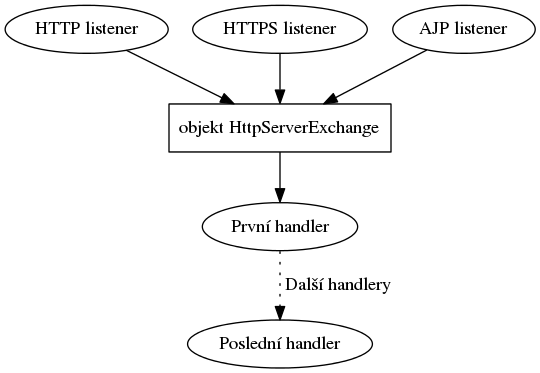
\includegraphics{dot/undertowArchitecture.png}}
                        \caption{Zjednodušená architektura serveru Undertow}
                        \label{imgUndertowArchitecture}
                    \end{center}
                \end{figure}
  
\begin{priklad} \label{prUndertow} Vytvoření jednoduché instance serveru Undertow
\begin{verbatim}
Undertow server = Undertow.builder()
  .addHttpListener(8080, "localhost")
  .setHandler(new HttpHandler() {
    @Override
    public void handleRequest(final HttpServerExchange exchange) 
        throws Exception {
      exchange.getResponseHeaders()
        .put(Headers.CONTENT_TYPE, "text/plain");
      exchange.getResponseSender().send("Hello World");
    }
  }).build();
server.start();
\end{verbatim}
\end{priklad}
                
                Třída \texttt{Undertow} reprezentuje instanci samotného
                webového serveru a~je ji nutné definovat prakticky vždy. Metodou
                \texttt{addListener} je přidán výše zmiňovaný \emph{listener}, který
                naslouchá na zvoleném síťovém rozhraní a~portu (při zvolení IP adresy 0.0.0.0 naslouchá
                na všech rozhraních). Tento jednoduchý příklad obsahuje pouze jeden \emph{handler} 
                přidaný metodou \texttt{addHandler}, který
                provádí veškerou činnost serveru a~tou je odpovídání na všechny požadavky jednotným textem. 
                Ve standardních aplikacích by následovalo volání dalšího \emph{handleru}.

            \subsubsection{Servlet kontejner}
                Servlet kontejner obsažený v~serveru Undertow je tvořen již implementovaným
                řetězcem \emph{handlerů}, které poskytují potřebné funkcionality odpovídající specifikaci.
                Pro nastavení základní funkcionality kontejneru existuje vysokoúrovňové rozhraní,
                ale opět je možné jeho funkce upravit nebo rozšířit pomocí vlastních \emph{handlerů}. 

                Při inicializaci servlet kontejneru se nastavují požadované funkce v~entitě \texttt{DeploymentInfo}
                a~až po jeho kompletním nastavení se provede vytvoření řetězce \emph{handlerů}, což
                dává prostor k~vnitřním optimalizacím. 
                Základní činností je potřeba nastavit prvky webové aplikace, které jsou definovány v~souboru web.xml (viz. kapitola \ref{kapWebXml}).
                Pro nastavení většiny možných prvků tohoto souboru je
                definováno několik statických metod ve třídě \\\texttt{io.undertow.servlets.Servlets}, které    %TODO check zalomení
                pomáhají servlet kontejner patřičně nastavit.

                Nastavení jednoduchého servlet kontejneru je demonstrováno na příkladu \ref{prServlet}.

\begin{priklad} \label{prServlet} Konfigurace jednoduchého servlet kontejneru
\begin{verbatim}
DeploymentInfo servletBuilder = Servlets.deployment()
    .setContextPath("/myapp")
    .setDeploymentName("test")
    .addServlets(
        Servlets.servlet("MessageServlet", MessageServlet.class));

DeploymentManager manager = Servlets.defaultContainer()
    .addDeployment(servletBuilder);
manager.deploy();
HttpHandler httpHandler = manager.start();
\end{verbatim}
\end{priklad}
                V~první části ukázky je vytvořená instance \texttt{DeploymentInfo}, která bude obsahovat jednoduchou konfiguraci
                s~jediným servletem. Následně pomocí proběhne přidání do výchozího kontejneru a~pomocí volání metody \texttt{deploy}
                se vytvoří celý řetězec \emph{handlerů}, které budou poskytovat požadovanou funkčnost.
                
                Celý proces je zakončen voláním metody \texttt{start}, kdy proběhnou poslední nastavení a~obdržíme 
                vstupní \emph{handler} celého servlet kontejneru.
                Poté jej lze nastavit jako vstupní \emph{handler} celé aplikace
                (viz metoda \texttt{addHandler} v~příkladu \ref{prUndertow}), ale také mu může předcházet několik jiných handlerů,
                což je typičtější případ.


            \subsubsection{Pokročilá konfigurace servlet kontejneru}
                Potřebných či možných nastavení servlet kontejneru je celá řada. Z~těch nejdůležitějších stojí za zmínku 
                správa zdrojů (angl. \emph{resource management}), nastavení autentizace a~zabezpečení servlet kontejneru
                a~úprava činnosti kontejneru pomocí vložení vlastních \emph{handlerů} do posloupnosti \emph{handlerů},
                která je vytvářena před jeho spuštěním.

                Pro správu zdrojů je nutné vytvořit instanci rozhraní \texttt{ResourceManager}, jinak kontejner při 
                každém požadavku na zdroj žádný nenajde (zjištěno ze zdrojových kódů). Je možné vytvořit si vlastní
                implementaci pro správu zdrojů nebo použít jednu z~implementací, které Undertow obsahuje:

                \begin{itemize}
                    \item \texttt{FileResourceManager} -- spravuje zdroje z~určené složky souborového systému
                    \item \texttt{ClassPathResourceManager}  -- spravuje soubory, které se nacházejí na \emph{classpath} kontejneru 
                        (cesta ke knihovnám určená při spuštění programu)
                    \item \texttt{CachingResourceManager} -- zastřešuje jinou implementaci správce zdrojů a~pro
                        urychlení pracuje jako vyrovnávací paměť (angl. cache)
                \end{itemize}

                %TODO pořádně zkontrolovat význam či přepracovat, přidat něco o securiy-constraints?
                Servlet kontejner může poskytovat dva základní typy zabezpečení. 
                První možností je poskytovat autentizaci v~případech, které uživatel deklaruje v~souboru
                \emph{web.xml}. Při tomto způsobu kontejner kontroluje příchozí požadavky a~v~případě
                potřeby požádá uživatele o~autentizaci. Pro správnou funkčnost tohoto způsobu zabezpečení
                je potřeba vytvořit objekt \texttt{LoginConfig} \cite{undertowServletSecurity} (odpovídající
                nastavení části \emph{login-config} ve \emph{web.xml} a~vytvořit vlastní implementaci
                rozhraní \texttt{IdentityManager}. Tato instance na základě požadavku rozhooruje, zda
                uživatel byl rozpoznán (a~případně jej blíže identifikuje) nebo zamítne požadavek na autentizaci.
                
                Druhou možností je definovat
                libovolný počet instancí rozhraní \texttt{AuthenticationMechanism}. Každý příchozí požadavek
                je následně prochází každou instatncí a~její základním činností je určit, zda požadavek má
                mít umožněn přístup do kontejneru nebo ne. Bližší informace lze nalézt v~dokumentaci z~níž
                byly čerpány informace v~této kapitole \cite{undertowDeployment}, \cite{undertowSecurity}.

                \medskip
                Upravit činnost servlet kontejneru je navíc možné tak, že se do něj vloží vlastní instance
                \emph{handlerů} a~ty libovolně upravují příchozí požadavky. Samotné vložení
                není možné provést přímo, protože servlet kontejner se sestavuje automaticky na základě
                definovaných vlastností. Je tedy nutné zaobalit handler do instance rozhraní \texttt{HandlerWrapper},
                který toto vložení umožní. Tato instance umožní následné vložení \emph{handleru} do řetězce \emph{handlerů}
                v~kontejneru. Je možné vložit \emph{handler} před vykonáním všech \emph{handlerů} serveru, po
                nastavení kontextu požadavku a~po vykonání všech handlerů před spuštěním kódu uvnitř uživatelského 
                servletru \cite{undertowDeployment}.
 
        
        \subsection{Srovnání serverů Undertow a~Jetty}\label{srovnani}
            Stávající servlet kontejner v~Jenkins CI je sice tvořen
            kombinací kontejneru Winstone a~serveru Jetty, ale veškerou
            časově kriticky náročnou práci při běhu aplikace vykonává server
            Jetty. Proto pokud chceme srovnávat původní a~plánované řešení servlet kontejneru
            v~Jenkins CI, tak bychom měli srovnávat server Jetty se serverem Undertow.

            \medskip
            Budeme tedy srovnávat servery Undertow a~Jetty, jejich výhody a~nevýhody
            vzhledem k~využití v~systému Jenkins CI:
            \begin{itemize}
                \item {\textbf{Rychlost:} Server Undertow je sice nový, ale už přesto existují
                    testy v~kterých se ukázal být výkonnější než server Jetty. V~tomto           
                    testování\footnote{Porovnání rychlosti, odezvy a~celkové výkonnosti serverů Undertow, Jetty a~jiných: 
                    \\\texttt{http://www.techempower.com/benchmarks/\#section=data-r8\&hw=ec2\&test=plaintext}}
                    byl server Undertow v~některých případech byl server 
                    Undertow i~3,5 krát rychlejší než server Jetty v~počtu zpracovaných 
                    požadavků za jednotku času. Při porovnávání doby odezvy serveru na požadavek 
                    dosáhl server Undertow až třetinového času než server Jetty. 
                    
                    Naopak při některých
                    jiných konfiguracích byl rychlejší server Jetty a~proto nelze definitivně určit,
                    který server je rychlejší a~podstatné je také způsob využití serveru. 
                    Dalším důležitým faktem je, že v~Jenkins CI není využita nejnovější verze serveru
                    Jetty (verze 9), ale jeho nižší verze 8, protože Jenkins CI aktuálně využívá
                    starší verzi jazyka Java (verzi Java 6).
                    
                    Lze tedy usuzovat, že server Undertow má potenciál být výkonnějším.
        
                    V~rámci této práce bylo provedeno vlastní základní testování 
                    obou těch serverů a~to ve vztahu přímo k~systému Jenkins CI. Tímto testováním
                    se zabýcá kapitola \ref{kapPerformance}, kde jsou porovnávány 
                    implementace servlet kontejneru s~využitím serveru Jetty a~nové implementace 
                    postavené na serveru Undertow.
                    }

                \item{\textbf{Spolehlivost:} Dalším důležitým aspektem je spolehlivost daného serveru. 
                        Server Jetty má za sebou již dlouhou historii a~je integrován ve velkém množství
                        různých aplikací\footnote{Aplikace, které využívají server Jetty: \texttt{http://www.eclipse.org/jetty/powered/}},
                        což mu dodává velkou důvěryhodnost a~lze očekávat, že bude pracovat velmi 
                        spolehlivě. 
                        
                        U~serveru Undertow byla dokončena první finální verze teprve nedávno,
                        takže lze předpokládat, že může obsahovat ještě drobné nedostatky,
                        které budou časem opravovány. Jelikož tento server je integrován
                        v~novém aplikačním serveru WildFly 8, tak lze předpokládat,
                        že postupem času bude také velmi spolehlivý. 
                        Nicméně v~tomto aspektu je server Jetty zřejmě 
                        aktuálně lepší.}

                %Tato část by měla být pečlivě překontrolována
                \item{\textbf{Konfigurovatelnost:} Server Undertow je velmi flexibilní a~způsob
                    jeho návrhu, který byl popsán výše, umožňuje provádět mnoho různých úpravy 
                    své činnosti dle potřeby a~využít pouze ty části, které potřebujeme.
                    Tato filozofie je velmi blízká filozofii projektu Jenkins CI. 
                    
                    Server Jetty
                    je oproti tomu robustnější a~rozsáhlejší, ale neumožňuje tak velké přizpůsobování potřebám
                    uživatele jako například využití jen několika malých částí jeho funkčnosti či jejich
                    kombinování. }


                \item{\textbf{Snadnost použití:}}                      
                    Server Jetty má již dlouhou historii a~je v~něm vše pečlivě dokumentováno
                    a~to jeho využití pro uživatele činí poměrně snadným. Podstatnou výhodou je, že
                    server Jetty poskytuje velké množství vysokoúrovňových rozhraní
                    pro různé konfigurace serveru.
                    
                    Jelikož je server Undertow velmi mladým projektem a~není tolik ustálený, 
                    tak postrádá některé věci,
                    které jsou u~serveru Jetty samozřejmostí. 
                    Dokumentace k~serveru
                    Undertow je poměrně strohá, místy ne úplně přesná a~stále se vyvíjí. 
                    Jeho velká flexibilita při konfiguraci s~sebou nese i~jisté nevýhody
                    a~tím je právě jednoduchost jeho použití. Další nepříjemností je, že není
                    dostupné tolik propracované rozhraní pro konfiguraci jako u~serveru Jetty,
                    což lze opět přičítat délce trvání projektu.

                    Je zjevné, že využití serveru Jetty je podstatně jednodušší než je tomu
                    u~serveru Undertow. Nicméně tato skutečnost je jen překážkou pro provedení
                    integrace, ale následně nemusí činit další problémy a~nijak neovlivňuje
                    funkčnost výsledné aplikace.

            \end{itemize}
        

%%%%%%%%%%%%%%%%%%%%%%%%%%%%%%%%%%%%%%%%%%%%%%%%%%%%%%%%%%%%%%%%%%%%%%%%%%%%%%%%%%%%%%%%%%%%%%%
%%%%%%%%%%%%%%%%%%%%%%%%%%%%%%%%%%%%%%%%%%%%%%%%%%%%%%%%%%%%%%%%%%%%%%%%%%%%%%%%%%%%%%%%%%%%%%%
%%%%%%%%%%%%%%%%%%%%%%%%%%%%%%%%%%%%%%%%%%%%%%%%%%%%%%%%%%%%%%%%%%%%%%%%%%%%%%%%%%%%%%%%%%%%%%%
%%%%%%%%%%%%%%%%%%%%%%%%%%%%%%%%%%%%%%%%%%%%%%%%%%%%%%%%%%%%%%%%%%%%%%%%%%%%%%%%%%%%%%%%%%%%%%%
%%%%%%%%%%%%%%%%%%%%%%%%%%%%%%%%%%%%%%%%%%%%%%%%%%%%%%%%%%%%%%%%%%%%%%%%%%%%%%%%%%%%%%%%%%%%%%%
\chapter{Analýza současného stavu servlet kontejneru a~návrh integrace}
    Tato kapitola se zabývá důkladnější analýzou a~zkoumáním architektury aplikace Jenkins~CI
    z~pohledu jejího vestavěného kontejneru a~jeho možných úprav (kapitola \ref{secArchitecture}). 
    Jsou konkretizovány jednotlivé činnosti, které současný servlet kontejner provádí
    a~které musí nová implementace také poskytovat (kapitola \ref{secKompatibilita}).
    Poslední část této kapitoly diskutuje možné varianty integrace serveru Undertow do Jenkins CI,
    jejich výhody a~nevýhody (kapitola \ref{secNavrh}). Jako výstup této analýzy je zvolen způsob integrace, jehož
    implementací se zabývá následující kapitola \ref{kapImpl}.

    Jelikož k~této problematice je minimum oficiální zdrojů, které by danou problematiku blíže popisovaly, 
    tak převážná část zde uváděných informací byla čerpána přímo ze zdrojových kódů aplikace a~komponent Jenkins CI.
    Na jejich základě byla prováděná analýza současného stavu servlet kontejneru v~aplikaci a~jeho architektury.
    
    \section{Aktuální stav architektury servlet kontejneru v~Jenkins~CI}\label{secArchitecture}
        V~následujících dvou podkapitolách je blíže analyzována architektura
        Jenkins CI z~pohledu servlet kontejneru. Tato analýza je velmi důležitá
        pro pochopení návazností jednotlivých komponent, které musely být v~rámci integrace upravovány.

        Jak již bylo uvedeno v~kapitole \ref{vyvojWinstone}, současný servlet kontejner 
        v~Jenkins CI se skládá z~nástojů Winstone a~Jetty, které byly také popisovány
        v~předchozích kapitolách. Velká část servlet
        kontejneru Winstone byla odstraněna a~zůstala pouze část, která
        provádí zpracování vstupních parametrů po spuštění aplikace, a~různé menší části
        vykonávající pomocné činnosti jako je loggování, rozbalování archivu apod. Činnost webového serveru, servlet kontejneru
        a~věci s~tím spojené vykonává server Jetty.
        

        \subsection{Architektura Jenkins CI z~pohledu servlet kontejneru} 
            Na vysoké úrovni pohledu lze architekturu serveru Jenkins CI rozdělit do tří částí:
            
            \begin{itemize}
                \item{\textbf{Jádro aplikace}, do kterého patří nejnutnější základní komponenty systému
                    a~části, které jsou pro Jenkins CI specifické a~nezbytné pro jeho běh. 
                    Vývoj těchto komponent je hlavní činností v~rámci celého projektu Jenkins CI.}

                \item{\textbf{Přídavné moduly} aplikace, které jsou do ní dynamicky přidávány jako archivy Java programů
                    \texttt{.jar}. Většina těchto součástí je nutná pro standardní běh aplikace a~je s~nimi aplikace
                    běžně dodávána (teoreticky lze
                    aplikaci spustit např. bez servlet kontejneru pomocí aplikačního serveru, ale toto je spíše ojedinělý případ). 
                    
                    Komponenty z~této kategorie pocházejí typicky z~externích projektů.
                    Spadá zde také servlet kontejner, který je aktuálně do aplikace
                    přidáván v~archivu s~názvem \\\texttt{winstone.jar}.}

                \item{\textbf{Rozšiřující moduly} (angl. plugins) jsou samostatné menší programy, které nějakým
                    způsobem přidávají funkcionalitu serveru Jenkins CI. Typicky je jich dodáváno jen velmi málo
s~distribucí aplikace 
                    a~uživatel si je může stáhnout nebo si nějaký vlastní modul vytvořit.
                    
                    Samotná aplikace se dodává jen s~těmi nejnutnějšími součástmi a~ponechává na uživatelích, které
                    další funkcionality si do systému doinstalují. V~současné době již existují stovky takových
                    modulů, které jsou volně ke stažení. }
            \end{itemize}
            

            V~následujícím textu bude při popisu interních součástí zdrojových kódů použita notace
            ve tvaru \texttt{Název\_třídy::Název\_metody}.

            Architektura Jenkins CI z~pohledu servlet kontejneru je znázorněna na obrázku \ref{imgArchitekturaServlet}.
            Jsou zde zachyceny především komponenty, které přímo souvisejí s~jeho činností.

            \begin{figure}[h!t]
                \begin{center}
                    \scalebox{0.7}{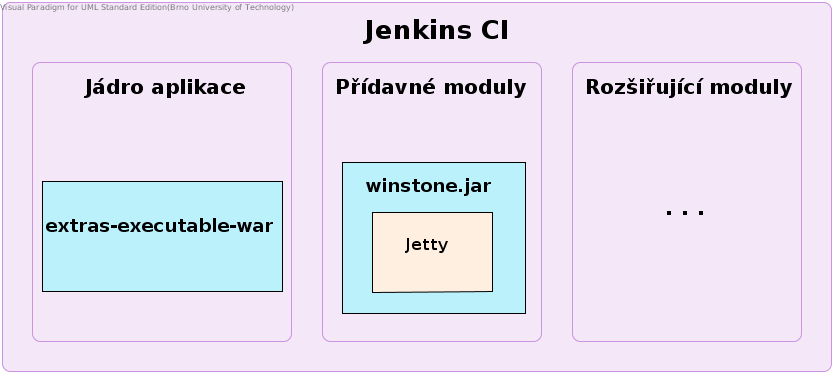
\includegraphics{img/architecture.png}}
                    \caption{Přehled architektury systému Jenkins CI z~pohledu vestavěného servlet kontejneru}
                    \label{imgArchitekturaServlet}
                \end{center}
            \end{figure}

            
            Archiv \texttt{winstone.jar} obsahuje servlet kontejner pro Jenkins CI. Název je nyní sice mírně matoucí
            (způsoben předchozí implementací), ale aktuálně jsou součástí tohoto archivu komponenty Winstone a~Jetty.

            Velmi podstatnou součástí aplikace z~pohledu servlet kontejneru je komponenta\\\texttt{extras-executable-war}. 
            Tato součást aplikace je sice malá, ale obsahuje metodu \texttt{main}, kterou se aplikace spouští 
            (pokud není spuštěna v~aplikačním serveru). Hlavním úkolem této komponenty je právě spustit 
            servlet kontejner a~tím spustit i~celou aplikaci. Tento proces spuštění aplikace je zobrazen
            na obrázku \ref{imgArchitekturaSpusteni}.

            Nejprve je spuštěna vstupní metoda celé aplikace \texttt{Main.java::main} z~komponenty\\\texttt{extras-executable-war}.
            Po počáteční inicializaci je předáno řízení aplikace metodě \\\texttt{Launcher.java::main}
            z~archivu \texttt{winstone.jar}, která provede nastartování
            a~zavedení servlet kontejneru. Následně je provedena inicializace a~spuštění
            jediného servletu aplikace Jenkins CI a~tím je servlet Stapler (bližší informace o~tomto
            servletu jsou v~kapitole \ref{secJenkinsArchitektura}). 
            Pokud se podaří úspěšně spustit tento servlet, tak je spuštění celé aplikace Jenkins CI z~pohledu
            servlet kontejneru úspěšně provedené a~aplikace běží.

            Zjištění, které komponenty má servlet kontejner při svém startu zavést,
            se nachází v~souboru \emph{web.xml}, což je standardní konfigurační soubor
            pro webové aplikace v~jazyce Java~EE. Může se zde nacházet také například
            konfigurace uživatelských účtů pro přístup k~aplikaci nebo~specifikování
            různých druhů přístupových práv.


            \begin{figure}[h!t]
                \begin{center}
                    \scalebox{0.64}{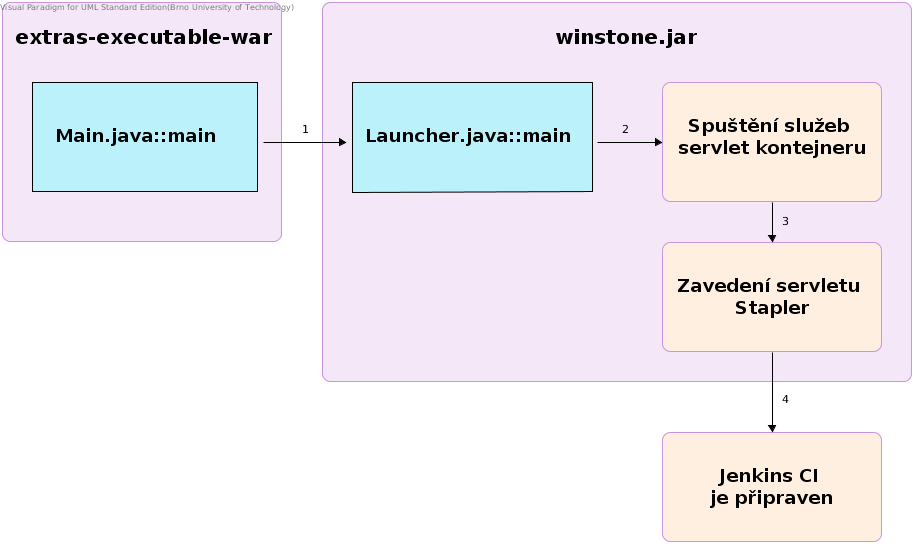
\includegraphics{img/jenkinsStart.png}}
                    \caption{Průběh spouštění aplikace Jenkins CI při spouštění pomocí vestavěného servlet kontejneru}
                    \label{imgArchitekturaSpusteni}
                \end{center}
            \end{figure}


        \subsection{Průběh komunikace prostřednictvím servlet kontejneru}
            Po úspěšném zavedení a~spuštění aplikace provádí servlet kontejner
            zpracovávání příchozích požadavků a~předává je aplikaci Jenkins CI. 
            Typický zjednodušený průběh komunikace servlet kontejneru s~aplikací je znázorněn
            na obrázku \ref{imgKomunikace}. 

            \begin{figure}[h!t]
                \begin{center}
                    \scalebox{0.64}{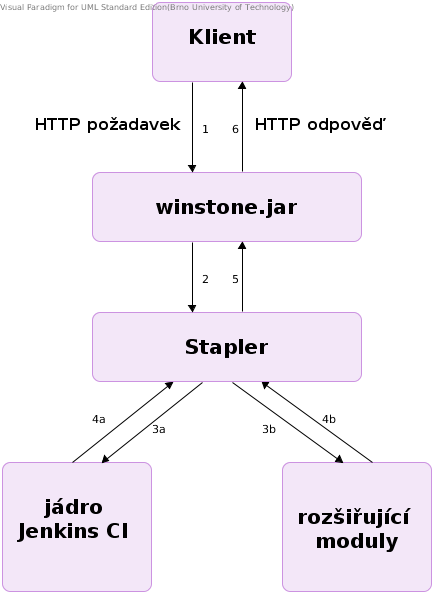
\includegraphics{img/jenkinsCommunication.png}}
                    \caption{Průběh komunikace aplikace Jekins CI prostřednictvím vestavěného servlet kontejneru}
                    \label{imgKomunikace}
                \end{center}
            \end{figure}

            Při komunikaci je příchozí HTTP požadavek zpracován pomocí servlet kontejneru 
            a~následně předán patřičnému servletu (dle nastavení pravidel pro směřování požadavků).
            Jelikož je v~aplikaci pouze jediný servlet Stapler, tak je požadavek předán jemu.
            Tato komponenta následně provede netriviálním způsobem rozhodnutí, které
            části aplikace předat požadavek k~vykonání  nebo zda náleží nějakému rozšiřujícímu modulu.
            Následně stejnou cestou probíhá zaslání HTTP odpovědi zpět klientovi.

            Byla zde zachycena pouze jedna z~možných činností
            servlet kontejneru a~tou je zpracovávání komunikace protokolem HTTP. 
            Další činnosti kontejneru budou rozebírány později.

 


    \section{Zpětná kompatibilita servlet kontejner v~Jenkins CI}   \label{secKompatibilita}
        V~této kapitole jsou blíže rozebírány a~analyzovány jednotlivé funkce servlet
        kontejneru v~Jenkins CI. Analýza jeho funkčnosti je zaměřena především na 
        návrh nového servlet kontejneru implementovaného pomocí serveru Undertow.
        Z~této kapitoly vyplynou hlavní požadavky, které je potřeba řešit 
        při samotné implementaci.

        Stávající servlet kontejner je v~Jenkins CI již dlouhou dobu
        a~mnoho uživatelů a~komponent systému přímo používá jeho specifické
        parametry, které pocházejí z~kontejneru Winstone~\cite{kohsukeTopic}. Nová implementace
        tudíž musí zachovat naprosto stejný formát parametrů, aby 
        se výměnou servlet kontejneru nestala část aplikace nebo rozšiřujících modulů nefunkční.
        Také je potřeba zachovat výchozí hodnoty jednotlivých parametrů.

        \subsection{Funkcionality servlet kontejneru} \label{kapFunkcionality}
            Při spouštění aplikace je před předáním řízení aplikace servlet kontejneru
            část parametrů zpracována komponentou \texttt{extras-executable-war} (blíže 
            rozebrána v~kapitole \ref{secArchitecture}) a~zbylé parametry jsou přímo
            předány servlet kontejneru, který podle nich nastaví svou činnost.
            Jednotlivé parametry zde nejsou rozebírány, ale následující analýza
            se zaměřuje především na klíčové body funkčnosti servlet kontejneru.

            Pro zachování zpětné kompatibility musí servlet kontejner v~aplikaci 
            Jenkins CI poskytovat především následující funkce:
            
            \begin{itemize}
                \item Provádět inicializaci a~spuštění webové aplikace, která je zabalená v~archivu \texttt{.war}
                    nebo je již rozbalená v~nějakém konkrétním adresáři na disku.
                
                \item Poskytovat možnost komunikace nešifrovaným protokolem HTTP, který je výchozím
                    komuničním protokolem v~serveru Jenkins CI.  Aplikace musí naslouchat na všech síťových rozhraních na portu 8080.
                
                \item Umožnit komunikaci šifrovaným síťovým protokolem HTTPS. V~Jenkins CI jsou dostupné 
                    3 způsoby inicializace šifrované komunikace, které se liší poskytnutými informacemi pro 
                    zabezpečení pomocí SSL:
                    \begin{itemize}
                        \item Zadáním certifikátu ve formátu PEM a~zároveň zadání privátního klíče serveru
                        \item Zadáním souboru, který obsahuje úložiště certifikátů (v~prostředí aplikací v~jazyce Java tzv. \emph{KeyStore}) a~zároveň zadání 
                            přístupového hesla k~tomuto souboru
                        \item Nezadání žádných bezpečnostních údajů. V~tom případě si servlet kontejner musí certifikát sám
                            vygenerovat a~pomocí něj inicializovat komunikaci. Je důležité dodat, že tento způsob
                            není pro běžné využití bezpečný a~je vhodné jej použít jen pro účely testování.
                    \end{itemize} 

                \item Komunikovat protokolem AJP13. Tento protokol se využívá při architektuře serveru,
                    kdy je HTTP server umístěn až za tzv. \emph{proxy} serverem. Typickým příkladem takového
                    \emph{proxy} serveru je program Apache\footnote{Webové stránky projektu Apache: 
                    \texttt{http://httpd.apache.org/}}. V~tomto případě je pro optimalizaci komunikace mezi HTTP serverem
                    a~\emph{proxy} severem využit protokol AJP13 \cite{ajp13Web}.

                \item Podporovat zabezpečení aplikace. Musí umožnit přihlašování uživatelů, správu přístupových práv a~rolí.
                    Tato problematika je blíže rozebírána v~následující kapitole~\ref{secSecurityArchitecture}.
                    
                \item Činnost servlet kontejneru může být ovlivňována pomocí komunikace přes síťové rozhraní zasláním zprávy
                    na speciální port. Při obdržení zprávy na tomto portu je potřeba umožnit ukončení nebo restartování aplikace.
                    Pro ukončení aplikace servlet kontejner očekává zprávu, která bude obsahovat pouze ASCII hodnotu číslice 0.
                    Restartování aplikace provede při obdržení zprávy s~ASCII hodnotou číslice 4. Jakékoliv
                    jiné zprávy než v~uvedeném formátu mohou být ignorovány.

                \item Zaznamenávat informace o~přístupech k~aplikaci. V~současném servlet kontejneru je možné zaznamenávat
                    údaje o~IP adrese, jménu uživatele (pro přístup do aplikace), času, cílové URL adrese, hodnotě 
                    kódu HTTP odpovědi a~o~hodnotách hlaviček \emph{Referer} a~\emph{User-Agent}, které jsou v~protokolu HTTP.
                    Při spuštění si uživatel může zvolit, které z~údajů si přeje zaznamenávat a~s~každý přístup poté 
                    servlet kontejner uchovává patřičné informace v~souboru na serveru.

            \end{itemize}
            

            Po integraci serveru Jetty do servlet kontejneru byla přidána ještě možnost
            komunikace protokolem SPDY. SPDY je nový síťový protokol aplikační vrstvy, který je
            navržen pro přenos obsahu webových stránek v~oblasti internetu. Jeho hlavní cílem je snížit odezvu stránek a~zdokonalit
            komunikaci, pro kterou již protokol HTTP není ideální \cite{spdyArticle}.
            Jeho využití v~budoucnu může přinést zrychlení aplikace, ale 
            tento protokol ještě není 
            v~Jenkins CI více využíván a~tudíž jeho podpora v~servlet kontejneru není pro činnost Jenkins CI zásadní~\cite{kohsukeTopic}.
        
        \subsection{Zabezpečení v~Jenkins CI} \label{secSecurityArchitecture}
            Zabezpečení serveru Jenkins CI z~pohledu autentizace a~autorizace je poměrně komplikované,
            ale pouze část se týká servlet kontejneru a~vyžaduje jeho činnost. 
            
            Autorizace a~autentizace je v~Jenkins CI založena na tzv. filtrech (angl. \emph{filters})
            (prvky webové aplikace upravující příchozí požadavky než je začne zpracovávat servlet) 
            a~na dalších metodikách, jejich většina není pro činnost servlet kontejneru podstatná~\cite{securityArchitectureJenkins}. 
            
            Kontrolu přístupu k~jednotlivým prvkům aplikace provádí 
            Jenkins CI samostatně, ale pro provádění autentizace využívá několik externích zdrojů. Pro nastavení autentizace
            poskytuje několik možností:

            \begin{itemize}
                \item Delegovat autentizaci na servlet kontejner
                \item Využít vlastní databázi uživatelů definovanou v~Jenkins CI
                \item Autentizovat uživatele pomocí LDAP serveru
                \item Delegovat autentizaci na databázi uživatelů v~operačním systému UNIX. Uživatelé 
                    se mohou přihlásit zadáním jejich přístupových práv do operačního systému. 
            \end{itemize}
            
            Pro podporu autorizace a~autorizace musí servlet kontejner zajistit správné zavedení aplikace a~nastavení
            všech položek souboru \emph{web.xml}, které se týkají bezpečnosti. Jedná se tedy především
            o~následující položky \cite{webXml}:

            \begin{itemize}
                \item \emph{security-role} umožňuje specifikovat různé typy rolí pro uživatele v~systému,
                    které je jim možné přidělit
                \item \emph{security-constraint} definuje části aplikace mají chráněný přístup a~role, které k~nim
                    mohou přistupovat. V~Jenkins CI je tato kontrola prováděná interně a~je specifikován
                    omezený přístup pouze k~přihlašovacímu formuláři.
                \item \emph{login-config} umožňuje určit způsob jakým se má po uživateli vyžadovat zadání přistupových
                    údajů, pokud přistupuje k~chráněnému zdroji, a~na jaké stránky má být přesměrován v~případě úspěchu
                    nebo neúspěchu pokusu o~přihlášení
            \end{itemize}
            
    
            \subsubsection{Autentizace pomocí servlet kontejneru}
                Jedním z~výše uvedených způsobů autentizace v~Jenkins CI je využít servlet kontejneru pro autentizaci.
                Princip tohoto způsobu autentizace v~Jenkins CI je znázorněn na obrázku \ref{imgSecurity}. 
                Tento způsob funguje následovně. Příchozí 
                požadavek je předán servlet kontejnerem do Jenkins CI k~normálnímu zpracování. 
                Pokud Jenkins CI zjistí, že uživatel
                není autentizován, tak pošle požadavek servlet kontejneru pro ověření uživatele. Servlet
                kontejner provede ověření a~vrátí buď identitu ověřeného uživatele nebo jeho ověření zamítne (z~důvodu
                neplatných přihlašovacích údajů).
                
                \begin{figure}[h!t]
                    \begin{center}
                        \scalebox{0.7}{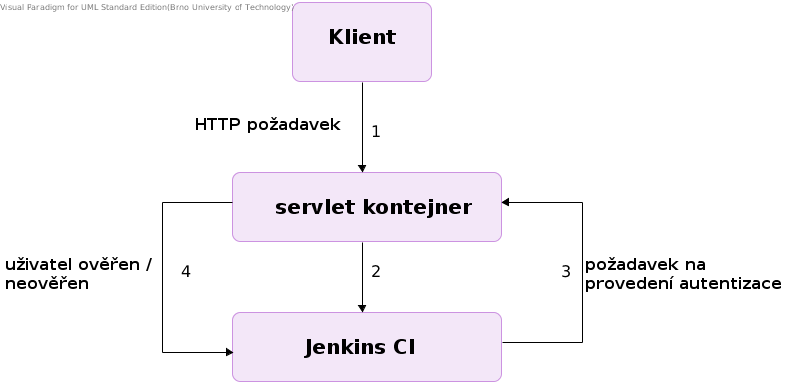
\includegraphics{img/jenkinsSecurity.png}}
                        \caption{Průběh autentizace uživatele pomocí servlet kontejneru}
                        \label{imgSecurity}
                    \end{center}
                \end{figure}

                Při použití tohoto způsobu autentizace je nutné správně nakonfigurovat servlet kontejneru před spuštěním.
                
                \begin{enumerate}
                    \item Definovat dostupné bezpečnostní role pro systém v~souboru \emph{web.xml}
                    \item Specifikovat uživatele systému s~jejich hesly a~s~libovolným výčtem rolí, které
                        jsou definovány v~prvním kroku
                \end{enumerate}

                V~aktuálním servlet kontejneru jsou předdefinovány dvě třídy, které provádějí autentizaci,
                a~je možné si zvolit jednu z~nich nebo si dodefinovat třídu vlastní.
                Dostupné třídy poskytují tyto dva způsoby přidávání uživatelů \cite{securityArchitectureWinstone}:

                \begin{itemize}
                    \item Přidávání uživatelů pomocí parametrů při spuštění příkazové řádky při spuštění servlet kontejneru 
                    \item Definování uživatelů v~XML souboru s~implicitním jménem \emph{users.xml} nebo 
                        lze specifikovat umístění tohoto souboru pomocí parametru. Formát položky
                        pro zadání uživatele je uveden v~příkladu \ref{prUsers}
                \end{itemize}

\begin{priklad} \label{prUsers}
    Formát položky XML souboru pro zadávání uživatelů v~aktuálním servlet kontejneru
\begin{verbatim}
    <user username="joe" password="doe" roles="user,admin" />
\end{verbatim}
\end{priklad}


    \section{Zjištěné problémy} \label{kapSpdy}
        Z~analyzování možností integrace vyplývá jeden problém.
        Při integraci serveru Jetty do Jenkins CI byla přidána
        možnost využít protokol SPDY, jehož implementace
        není v~současné době v~serveru Undertow dostupná. Nicméně tato možnost
        je zavedena jen krátce a~zřejmě ještě není využívána žádnými komponentami,
        takže by neměl být problém, kdyby nová implementace neobsahovala tuto volbu.
        
        Je důležité poznamenat, že základ implementace tohoto protokolu byl
v~serveru Undertow již proveden, ale ještě není začleněn do aktuální 
        verze. Takže z~dlouhodobého hlediska bude možné tento problém odstranit.

    \section{Návrh způsobu integrace serveru Undertow} \label{secNavrh}
        Na základě analýzy, která proběhla v~předchozích kapitolách,
        je v~této kapitole zvolen způsob
        integrace serveru Undertow do systému Jenkins CI. 
        Obě navržené možné varianty integrace jsou porovnány z~různých
        hledisek a~je zvolen způsob, kterým bude následně implementace provedena.

                
        \subsection{Varianty integrace}
            Pro integraci serveru Undertow do systému Jenkins CI jsou možné tyto dva přístupy:

            \begin{enumerate}
                \item{Nahrazení pouze serveru Jetty v~servlet kontejneru a~ponechání
                    zbytku implementace kontejneru Winstone, což by představovalo
                    pouze úpravy části stávajícího kódu. }

                \item{Nahrazení jak serveru Jetty tak kontejneru Winstone. 
                    Tento přístup v~podstatě znamená provedení celé implementace
                    servlet kontejneru pro Jenkins CI úplně znovu.}
            \end{enumerate}

            \noindent Obě varianty integrace mají své klady a~zápory. 
            Srovnáme je z~hlediska výkonu, proveditelnosti a~zpětné kompatibility
            implementace, abychom mohli následně zvolit vhodnější variantu:

            \begin{itemize}
                \item{\textbf{Srovnání výkonu:} V~první variantě integrace je ponechána stále
                 poměrně stará implementace kontejneru Winstone, která zřejmě stále ještě
                 obsahuje nepotřebné součásti. Samotný způsob inicializace není optimalizován
                 pro potřeby serveru Undertow, takže by mohlo docházet ke zbytečnému
                 zpomalování aplikace.
                 Nová implementace může být přímo optimalizována pro potřeby 
                 serveru Undertow a~poskytovat lepší výkon i~kratší dobu spuštění aplikace.}

                \item{\textbf{Srovnání proveditelnosti:} První varianta představuje provedení 
                    úprav pouze v~částech, kde je přímo integrován server Jetty, 
                    zatímco v~druhé variantě je potřeba provést znovu celou implementaci
                    integrace servlet kontejneru. 
                                         
                    V~tomto případě je úprava stávajícího kódu aplikace
                    zřejmě snazším přístupem a~také umožňuje provedení rychlejší
                    implementace, protože není nutné návrhovat celý modul,
                    ale pouze jeho části, a~je možné využít některé stávající části aplikace
                    jako zpracovávání parametrů, rozbalování archivů, apod.}

                \item{\textbf{Srovnání zpětné kompatibility:} Dosažení zpětné kompatibility
                    u~první varianty je snazší, jelikož jsou viditelná místa, která je 
                    potřeba znovu implementovat a~nezanedbat. Nicméně druhá varianta
                    nemá žádné faktické nevýhody, které by bránily dosažení 
                    stejné úrovně zpětné kompatibility jako u~první varianty.}

                \item{\textbf{Další hlediska:} Jelikož dlouhodobý vývoj servlet kontejneru
                    v~Jenkins CI je na okraji zájmu a~jsou prováděny především nejnutnější úpravy, 
                    tak celý kód poněkud zdegeneroval a~je obtížně čitelný. Toto
                    je u~\emph{open source} projektu velká závada 
                    a~může bránit dalším přispěvovatelům k~provádění potřebných změn.

                    Z~tohoto pohledu by nová implementace mohla přinést mnohem čitelnější
                    způsob řešení a~zbavit kód zbytečností z~původní realizace servlet kontejneru.}
            \end{itemize}



        \subsection{Zvolení způsobu integrace}
            Při výběru varianty integrace serveru Undertow do Jenkins CI byly zváženy
            výhody a~nevýhody, které byly popsány v~předchozí kapitole. Při nahrazení pouze serveru Jetty
            by provedení integrace zřejmě probíhalo podstatně snadněji než ve variantě druhé,
            ale z~kvalitativního pohledu se tato varianta jeví jako méně vhodná. 
            Hlavními 
            negativy jsou především potenciálně nižší výkonnost a~také špatná čitelnost
            zdrojových kódů.

            Při implementaci budou tedy nahrazeny obě komponenty stávajícího servlet kontejneru
            a~bude tudíž provedena celá implementace znovu s~využitím serveru Undertow. Tato
            varianta by měla přinést lepší čitelnost zdrojového kódu a~poskytnout 
            lepší výkonnost celé aplikace než druhá varianta.


            \medskip
            Architekturu spouštění a~integrace servlet kontejneru v~aplikaci není potřeba měnit a~při integraci bude
            zachován stávající stav tak, který byl popsán při analýze architektury (kapitola \ref{secArchitecture})
            Zvolený způsob integrace vyžaduje vytvoření úplně nového projektu a~jeho začlenění do stávající
            verze serveru Jenkins CI. Nový servlet kontejner musí být vyvíjen jako samostatný modul,
            který bude zabalen v~archivu \texttt{.jar}, aby jej bylo možné následně vložit jako externí modul do Jenkins CI.
            Pro spuštění nového servlet kontejneru
            je potřeba upravit modul \texttt{extras-executable-war} (viz kapitola \ref{secArchitecture}), který
            je vstupním bodem aplikace a~mimo jiné provádí spuštění servlet kontejneru.
            
            Hlavním cílem tohoto projektu je zachovat kompatibilitu s~aktuální verzí servlet kontejneru a~tudíž je 
            potřeba implementovat všechny podstatné funkcionality tak, jak byly popsány v~kapitole \ref{secKompatibilita}.
            












%%%%%%%%%%%%%%%%%%%%%%%%%%%%%%%%%%%%%%%%%%%%%%%%%%%%%%%%%%%%%%%%%%%%%%%%%%%%%%%%%%%%%%%%%%%%%%%
%%%%%%%%%%%%%%%%%%%%%%%%%%%%%%%%%%%%%%%%%%%%%%%%%%%%%%%%%%%%%%%%%%%%%%%%%%%%%%%%%%%%%%%%%%%%%%%
%%%%%%%%%%%%%%%%%%%%%%%%%%%%%%%%%%%%%%%%%%%%%%%%%%%%%%%%%%%%%%%%%%%%%%%%%%%%%%%%%%%%%%%%%%%%%%%
%%%%%%%%%%%%%%%%%%%%%%%%%%%%%%%%%%%%%%%%%%%%%%%%%%%%%%%%%%%%%%%%%%%%%%%%%%%%%%%%%%%%%%%%%%%%%%%
%%%%%%%%%%%%%%%%%%%%%%%%%%%%%%%%%%%%%%%%%%%%%%%%%%%%%%%%%%%%%%%%%%%%%%%%%%%%%%%%%%%%%%%%%%%%%%%
\chapter{Implementace}  \label{kapImpl}
    Tato kapitola popisuje způsob, jakým byla provedena samotná integrace serveru Undertow do Jenkins CI.
    Jednotlivé kroky zde popisované se přímo vážou k~informacím, které byly uvedeny v~předchozích kapitolách.

    

    
    \section{Základní informace}
        Integrace serveru Undertow do Jenkins CI zahrnovala vytvoření nového projektu, který 
        jsem pojmenoval \emph{Undertow4Jenkins}. 
        Jak vyplývá z~předchozích kapitol, tak program byl vytvořen v~jazyce Java a~jeho základ 
        tvoří server Undertow. 
        Z~důvodu kompatibility se serverem Jenkins CI musela být využita starší verze jazyka a~to verze 6.
        Pro správu a~překlad projektu bylo nutné použít program Maven. 
        
        Projekt Jenkins CI je umístěn na serveru GitHub v~několika oddělených repozitářích, které
        využívají verzovací program Git. Aby vývoj nového servlet kontejneru bylo možné následně předvést 
        komunitě Jenkins CI, tak byl tento projekt také verzován na serveru GitHub\footnote{Server GitHub je 
        dostupný na adrese: \texttt{https://github.com/}} 
        a~je uveřejněn pod licencí \emph{Apache License 2.0}\footnote{Text licence \emph{Apache license 2.0} je dostupný na: 
        \texttt{http://www.apache.org/licenses/LICENSE-2.0.html}}, takže je \emph{open source} projektem.

        Na počátku integrace bylo nutné vytvořit kopie (tzv. \emph{fork}) dvou repozitářů stávající implementace serveru Jenkins CI.
        Jedná se o~repozitář s~celým serverem\footnote{Adresa kopie repozitáře Jenkins CI: 
        \texttt{https://github.com/jbartece/jenkins}} a~také jeho modul 
        \\\texttt{extras-executable-war}\footnote{Adresa kopie modulu \texttt{extras-executable-war}:
        \texttt{https://github.com/jbartece/extras-executable-war} }.
        Vývoj nového servlet kontejneru probíhal na verzi \texttt{1.543} systému Jenkins CI, což byla nejnovější verze
        programu v~době, kdy započala práce na tomto diplomovém projektu. 
        
        \medskip
        Jelikož hlavním cílem projektu je dosáhnout zpětné kompatibility s~původní verzí servlet kontejneru,
        tak v~případě nejasného přístupu k~implementaci některých komponent byly studovány zdrojové kódy
        původní implementace a~nové servlet kontejner jim byl přizpůsobován. Tohoto přístupu bylo využito
        například při volbě šifrovacích protokolů pro nastavení komunikaci pomocí protokolu HTTPS nebo nastavení zaznamenávání
        příchozích požadavků.
        
     \section{Rozbor způsobu implementace}
        Tato kapitola se více zaměřuje na způsob, jakým byla implementace provedena. Jsou rozebrány nejdůležitější
        části implementace výsledného servlet kontejneru, způsob integrace do Jenkins CI
        a~celé jeho architektura. V~této kapitole se předpokládá, že čtenář je
        základním způsobem seznámen se servery Undertow a~Jenkins CI v~rozsahu, který byl popsán
        v~předchozích kapitolách.


        \subsection{Nahrazení původního servlet kontejneru}
            První krokem před započetím vývoje nového servlet kontejneru bylo zajištění vložení archivu \texttt{undertow4jenkins.jar} 
            do výsledného archivu \texttt{.war}.
            Jelikož je Jenkins CI překládán programem Maven, tak byla změněna závislost v~souboru \texttt{pom.xml} 
            (viz kapitola \ref{maven} o~programu Maven)
            z~původního kontejneru \emph{winstone} na nový projekt \emph{Undertow4Jenkins}.
            Nastavení této konfigurace je uvedeno na příkladu \ref{prDep}. Jedná se o~zvolenou identifikaci nového servlet
            kontejneru pro program Maven, který provede vložení archivu \texttt{.jar} do Jenkins CI ze svého lokálního repozitáře.

\begin{priklad} \label{prDep} Identifikace nového servlet kontejneru pro program Maven 
\begin{verbatim}
   <groupId>org.jenkins-ci</groupId>
   <artifactId>undertow4jenkins</artifactId>
   <version>0.1-SNAPSHOT</version>
   <classifier>jar-with-dependencies</classifier>
\end{verbatim}
\end{priklad}

            Po úspěšném vložení archivu nové implementace byl upraven modul \\\texttt{extras-executable-war}.
            Většina jeho činnost byla ponechána, ale bylo nahrazeno spuštění původního servlet kontejneru
            jeho novou implementací. Po takto provedeném nastavení byla práce zaměřena přímo na vývoj
            nového servlet kontejneru. 

        


        \subsection{Realizace základních funkcionalit}
            V~této kapitole jsou popsány klíčové části vytvořené aplikace a~způsob jakým byly implementovány. Většina těchto
            funkcionalit přímo koresponduje s~uvedenými požadavky na zachování kompatibility s~původní verzí, 
            které jsou popsány v~kapitole \ref{secKompatibilita}.
            Zde uváděné přístupy a~komponenty serveru Undertow jsou blíže rozebrány v~kapitole \ref{undertow}.

            %moznost pridat diagram aktivit s optional vetví činností, které se nemusí zadat
            Proces inicializace servlet kontejneru probíhá v~několika krocích, které na sebe
            navazují. V~následujícím přehledu jsou jednotlivé činnosti seřazeny tak, jak
            se po sobě vykonávají. 
            Část činností se provádí při každém spuštění servlet kontejneru,
            ale některé jsou volitelné a~spouštějí se pouze pokud jsou při spuštění
            zadány určité parametry. 

            \begin{enumerate}
                \item \textbf{Zpracování parametrů:} Jsou zkontrolovány zadané parametry
                    aplikace a~přítomnost povinných parametrů. Při spuštění aplikace
                    musí být zadán archiv \texttt{.war} s~aplikací nebo předána cesta
                    ke složce, ve které je tento archiv extrahován. 
                    Parametry aplikace
                    přesně odpovídají parametrům, které jsou dostupné v~nápovědě 
                    serveru Jenkins CI. 
                    
                    V~servlet kontejneru je dostupné velké množství parametrů
                    a~proto je jejich zpracování implementováno s~důrazem na obecnost a~jednoduché
                    přidávání nových parametrů. 
                    Pro přidání nového parametru stačí do třídy pro parametry přidat položku (tzv. \emph{field})
                    a~jeho datový typ (jsou podporovány datové typy \texttt{Boolean}, \texttt{String}, 
                    \texttt{Integer}) a~jeho zpracování bude probíhat patřičným
                    způsobem. K~dosažení této obecnosti bylo využito \emph{Java Reflection API}.
                    Jako podpora pro zpracování parametrů byla použita knihovna \emph{Apache
                    Commons CLI}\footnote{Knihovna \emph{Apache Commons CLI} je 
                    dostupná na: \texttt{http://commons.apache.org/proper/commons-cli/}}
                    
                \item \textbf{Příprava adresáře s~webovou aplikací:}  Webová aplikace
                    je předávána servlet kontejneru ve formě 
                    archivu \texttt{.war} (parametr \texttt{warfile}). Tento archiv je následně extrahován do 
                    adresáře, který je specifikovaný jako další parametr servlet kontejneru (parametr \texttt{webroot}).
                    
                    Načítání aplikace bylo provedeno obecně a~je ji možné spustit zadáním
                    pouze adresáře, kde je archiv již extrahován. Tyto možnosti mohou posloužit
                    např. při psaní testů.

                \item \textbf{Připravení načítání tříd:} Jsou vyhledány knihovny 
                    a~přeložené třídy aplikace ve standardních adresářích 
                    \texttt{/WEB-INF/lib} a~\texttt{/WEB-INF/classes}, které jsou definovaným
                    umístěním pro tyto zdroje (viz kapitola \ref{kapWebXml}). 
                    Na základě dostupných knihoven a~tříd je vytvořen instance třídy \texttt{URLClassLoader},
                    která provádí inicializaci a~zavádění tříd v~programu. 
                    
                    Tento zavaděč je potřebný
                    při vyhledávání tříd specifikovaných v~souboru \emph{web.xml} a~jeho instance
                    je předána serveru Undertow při inicializaci, aby bylo možné zavádět
                    potřebné součásti aplikace za běhu.

                \item \textbf{Analýza souboru web.xml:} Soubor \emph{web.xml} je 
                    zpracován za pomoci XML parseru \emph{StAX}, který je standardně dostupný v~knihovně
                    jazyka Java. Z~analyzovaného souboru jsou načteny potřebné informace pro inicializaci
                    Jenkins CI. Podpora všech možných konfigurací souboru \emph{web.xml} je velmi rozsáhlá
                    a~proto byla implementována pouze podpora těch konfigurací, které jsou
                    v~systému Jenkins CI využité. Nicméně toto zpracování bylo vytvořeno obecně 
                    a~je možné jej rozšířit o~další konfigurace, což může být předmětem dalšího vývoje,
                    ale není to nezbytné pro běh serveru Jenkins CI.
                
                \item \textbf{Nastavení servlet kontejneru v~Undertow:} V~tomto kroku
                    jsou již připraveny všechny pomocné informace pro nastavení servlet kontejneru
                    a~spuštění Jenkins CI. Nejprve jsou všechny načtené konfigurace ze souboru \emph{web.xml}
                    nastaveny v~třídě \texttt{DeploymentInfo}, která reprezentuje data pro vytvoření servlet
                    kontejneru. Při konfiguracích jsou načítány třídy z~archivu aplikace pomocí zavaděče vytvořeného
                    v~předcházejících krocích.

                    Jednou ze standardních konfigurací servlet kontejneru je definování typů souborů tzv.
                    \emph{MIME}. V~původním servlet kontejneru bylo automaticky načítáno téměř tisíc těchto mapování
                    a~proto jsou tyto hodnoty načítány i~v~nové implementaci.
                    
                    Pro správu statických zdrojů Jenkins CI je vytvořena instance třídy \\\texttt{FileResourceManager}
                    tak, aby poskytovala zdroje z~adresáře s~extrahovaným archivem aplikace. Tato třída
                    byla navíc zaobalena ještě objektem třídy \\\texttt{CachingResourceManager}, která
                    pracuje jako vyrovnávací paměť (angl. \emph{cache}) a~poskytuje lepší výkonnost
                    při práci se zdroji.


                \item \textbf{Nastavení správy uživatelských účtů (volitelné):} Základem autentizace
                    uživatelů je třída, která implementuje rozhraní \texttt{IdentityManager}, a~ta musí
                    být předána Undertow před jeho spuštěním. 
                    V~souladu s~původní implementací servlet kontejneru byly vyvořeny dvě třídy pro autentizaci, které
                    se liší pouze způsobem jak načítají data o~uživatelích (uživatelské jméno, heslo a~jeho role):
                    \begin{itemize}
                        \item \texttt{ArgumentsIdentityManager} -- načítá informace o~uživatelích z~parametrů předáných
                            při spuštění aplikace
                        \item \texttt{FileIdentityManager} -- načítá informace o~uživatelích z~XML souboru s~definovaným formátem 
                            (viz kapitola \ref{secSecurityArchitecture})
                    \end{itemize}

                    Jelikož tyto třídy se liší pouze způsobem načítání uživatelů, tak byly ostatní činnosti potřebné pro
                    autentizaci uživatelů extrahovány 
                    do abstraktní třídy \\\texttt{GenericIdentityManager}, kterou rozšiřují.
                        
                    Do servlet kontejneru je možné přidat vlastní třídu pro autentizaci pomocí parametru,
                    který definuje její plně kvalifikované jméno. Je pouze nutné, aby tato třída implementavala
                    rozhraní \texttt{IdentityManager}.

                    Volba třídy pro autentizaci se provádí zadáním jejího plně kvalifikovaného jména, což
                    je způsob, který musel být zachován v~souladu s~původní implementací servlet kontejneru. 
                    Zde ovšem vzniká problém, protože v~původní implementaci byla jiná struktura balíků
                    a~názvy tříd. Z~tohoto důvodu je v~aplikaci kontrolováno, zda nebylo zadáno
                    jméno třídy z~původní implementace a~je případně nahrazeno za třídu v~současné implementaci.
                    Stejný přístup byl použit při externím zadávání tříd v~následujcím bodu.
                
                \item \textbf{Nastavení zaznamenávání příchozích požadavků (volitelné):}
                     Tato funkcionalita je řešena přidáním vlastního \emph{handleru} na konec řetězce 
                     těsně před tím než je vyvolán samotný servlet. V~servlet kontejneru je 
                     vytvořena jedna třída zajišťující tuto činnost (odpovídající implementaci v~původním
                     kontejneru), ale je opět možné přidat vlastní implementaci. Toto přidání
                     je řešeno obdobně jako bylo popsáno v~předchozím bodě, ale
                     třída musí implementovat rozhraní \texttt{AccessLoggerHandler}.
                     
                
                \item \textbf{Konfigurace webového serveru:} 
                    Po inicializaci servlet kontejneru zbývá patřičně nastavit 
                    samotný webový server. Jsou incializovány konektory pro uživatelem zadané
                    protokoly pro komunikaci (dostupnými protokoly jsou HTTP, HTTPS a~AJP). 
                    Jsou implementovány tři způsoby nastavení šifrované komunikace pomocí SSL, jejichž 
                    implemetace je založena na implementaci v~původním servlet kontejneru
                    a~odpovídá popisu v~kapitole \ref{kapFunkcionality}.
                    
                    Pokud uživatel specifikoval při spuštění požadavek (parametr \texttt{prefix}), 
                    aby  URL adresa aplikace začínala 
                    nějakým daným řetězecem, tak je tento požadavek implementován
                    přidáním \emph{handleru} \texttt{RedirectHandler} jako vstupního \emph{handleru}
                    celé aplikace.

                    Provedním těchto posledních konfigurací je webový server i~servlet kontejner
                    plně inicializován a~následně je spuštěn.
                
                \item \textbf{Vytvoření řídícího portu (volitelné):} 
                    V~době kdy již províhá spouštění webového serveru, 
                    tak je možné vytvořit rozhraní pro ukončení nebo restart aplikace.
                    Je vytvořený standardní síťový \emph{socket} a~až do ukončení aplikace
                    na něm naslouchá příchozím požadavkům (parametr \texttt{controlPort}). Protokol, který akceptuje je popsaný
                    v~kapitole \ref{kapFunkcionality}.

            \end{enumerate}




        \subsection{Popis struktury programu}
            Tato kapitola se blíže zabývá vnitřní strukturou programu a~jejím cílem je zjednodušit 
            čtenáři orientaci ve zdrojových kódech aplikace.
            Popis všech tříd aplikace by byl příliš rozsáhlý a~neposkytoval by ucelený přehled o~aplikaci.
            Budou tedy popsány pouze balíky, do kterých je aplikace rozdělena
            a~tří nejdůležitější třídy, které jsou významné tím, že spojují jednotlivé části aplikace.
            Struktura aplikace je znázorněna na obrázku \ref{imgPackage}.
                    
            \begin{figure}[h!t]
                \begin{center}
                    \scalebox{0.7}{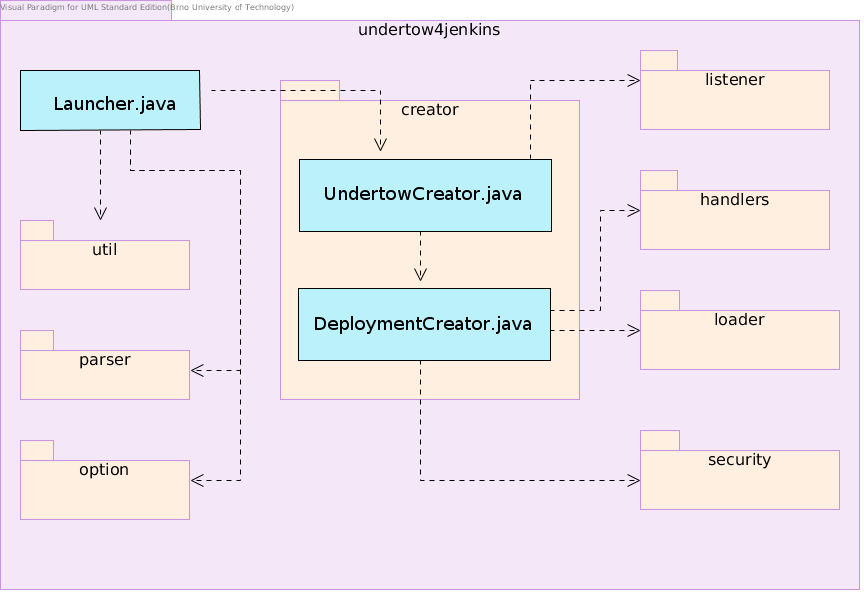
\includegraphics{img/package.png}}
                    \caption{Diagram balíků, rozšířený o~tři nejdůležitější třídy, který zachycuje architekturu servlet kontejneru}
                    \label{imgPackage}
                \end{center}
            \end{figure}

            Hlavními třídami architektury programu jsou třídy:
            \begin{itemize}
                \item \texttt{Launcher} -- vstupní bod aplikace obsahující metodu \texttt{main}. 
                    Zajišťuje kontrolu celého běhu servlet kontejneru. 

                \item \texttt{UndertowCreator} -- stará se o~inicializaci webového serveru
                    a~konfiguraci servlet kontejneru deleguje na třídu \texttt{DeploymentCreator}.

                \item \texttt{DeploymentCreator} -- zajišťuje inicializaci servlet kontejneru 
            \end{itemize}


            V~následujícím výčtu jsou stručně popsány balíky aplikace.
            Některé obsahují i~větší množství tříd a~proto je uvedeno pouze o~jaké činnosti
            se třídy v~daném balíku starají:
            \begin{itemize}
                \item \texttt{option} -- zpracování parametrů a~jejich reprezentace za běhu programu
                \item \texttt{parser} -- načtení souboru \emph{web.xml} a~reprezetace načtených hodnot
                \item \texttt{creator} -- vytvoření webového serveru a~servlet kontejneru pomocí Undertow
                \item \texttt{listener} -- vytvoření konektoru pro síťové protokoly HTTP, HTTPS a~AJP
                \item \texttt{handlers} -- vlastní vytvořené handlery pro běh aplikace
                \item \texttt{loader} -- inicializace servlet kontejneru na základě načtených informací ze souboru \emph{web.xml}
                \item \texttt{security} -- zajištění podpory autentizace uživatelů
                \item \texttt{util} -- zpracování webového archivu a~načítání informací z~konfiguračních souborů
            \end{itemize}




    \section{Řešené problémy při implementaci}
        Při implementaci jsem se potýkal s~nedostatečným komentováním zdrojových kódů serveru Undertow.
        Velká část serveru je naprosto nedostatečně komentovaná a~největším problémem je, že
        není komentované ani veřejné rozraní API. 
        Dokumentace projektu v~průběhu implementace teprve postupně vznikala a~navíc se zaobírá pouze popisem jednotlivých součástí,
        ale implementační detaily jsou rozebírány jen v~některých částech.
        Z~těchto důvodů bylo během implementace nutné velmi často zkoumat a~analyzovat přímo zdrojové kódy serveru Undertow
        a~někdy i~napsané integrační testy, které umožňují lépe pochopit některé typy konfigurací (např. vytvoření podpory autentizace
        pomocí instance rozhraní \texttt{Identity Manager}).

        Implementace některých částí aplikace byla podstatně komplikovanější oproti původní verzi servlet kontejneru
        a~očekáváním na začátku projektu. Server Undertow 
        neposkytuje některé standardní funkcionality pro integraci servlet kontejneru. Mezi nejvýznamnější patří nutnost
        zpracování souboru \emph{web.xml} a~nastavení dle něj servlet kontejneru nebo například nutnost 
        provádět zavádění tříd servletů (tzv. \emph{classloading}). V~aplikaci Jetty lze provést načtení 
        souboru \emph{web.xml} pomocí jediného volání metody serveru.

        
    \section{Omezení aplikace}
        Veškerá podstatná funkčnost servlet kontejneru byla zachována a~při testování nebyly odhaleny žádné chyby,
        ale některé nedůležité parametry nebyly implementovány. Aby nedocházelo
        k~problémům s~kompatibilitou (např. při spouštění staršími skripty), tak program zadání těchto
        parametrů akceptuje, ale pouze vypíše varování, že nejsou podporovány a~dále je ignoruje.
        
        \medskip
        \noindent Nepodporovanými parametry jsou:
        \begin{itemize}
            \item Parametr \texttt{spdy}, který umožňoval zapnutí podpory komunikace pomocí protokolu SPDY. Tento parametr
                nebyl implementován, jelikož v~aktuální verzi Undertow není ještě podporován, ale zřejmě
                brzy bude přidán (viz kapitola \ref{kapSpdy}.

            \item Skupina parametrů \texttt{httpDoHostnameLookups}, \texttt{httpsDoHostnameLookups}, \\\texttt{handlerCountStartup},
                \texttt{logThrowingLineNo}, které zůstaly v~kontejneru jako pozůstatek z~původní implementace, ale po integraci
                serveru Jetty do servlet kontejneru se přestaly využívat.

            \item Parametry \texttt{webappsDir} a~\texttt{hostsDir} byly v~aktuálním servlet kontejneru implementovány
                a~sloužily ke spuštění více webových aplikací v~servlet kontejneru. Server Jenkins CI má omezení,
                že může současně běžet na jednom počítači pouze jeho jediná instance. 
                Jelikož tento servlet kontejner je určen pouze pro Jenkins CI, tak jejich implementace nebyla smysluplná,
                protože by tyto parametry nemohly být využity pro jeho spuštění.

            \item Parametr \texttt{handlerCountMaxIdle} umožňoval určit maximální počet vláken servlet kontejneru, 
                které aktuálně neprováděly žádnou činnost. V~původní implementaci byla vlákna pro práci servlet kontejneru
                inicializována ručně instance rozhraní \\\texttt{ExecutorService} ze standardní knihovny. Jelikož
                tato možnost v~serveru Undertow nebyla, tak byla správa vláken ponechána ve výchozím stavu,
                protože tento parametr nemá zásadní vliv na zachování zpětné kopatibility.

            \item Parametry \texttt{debug} a~\texttt{logThrowingThread}, které pouze upravovaly vypisování průběhu
                běhu aplikace, ale nemají žádný vliv na jeho funkčnost. Jejich implementace může být předmětem dalšího
                vývoje.
        \end{itemize}
        
        
        Při implementaci dvou parametrů \texttt{httpKeepAliveTimeout}, \texttt{httpsKeepAliveTimeout}, které slouží 
        k~určení doby uchovávání aktivních spojení při komunikaci (hodnota \emph{keep-alive}), nebylo možné jednoduchým způsobem
        nastavit chování serveru jako u~původní verze. U~původní verze bylo možné provést nastavení zvlášť pro
        protokol HTTP i~HTTPS, ale při standardním využití serveru Undertow lze nastavit tuto hodnotu pouze pro celý
        server a~tedy společnou pro oba protokoly. 
        
        Existuje možnost nevyužít veřejné API pro sestavení serveru 
        a~provést podstatně komplikovanější variantu jeho inicializace při které by bylo možné nastavit tyto hodnoty \cite{undertowAssembly}.
        Tento přístup by byl překážkou při dalším vývoji servlet kontejneru, protože by bylo nutné tento
        kód upravovat s~přicházejícími novými verzemi Undertow (např. při přidání podpory SPDY). 
        Z~těchto důvodů bylo zvoleno kompromisní řešení, kdy je možné zadat hodnoty těchto parametrů, ale
        jsou využity pro celý server. Pokud jsou zadány oba parametry, tak je jako prioritní zvolen
        parametr pro protokol HTTP. Tato úprava by neměla negativně ovlivnit chování serveru a~pokud
        by se servlet kontejner ustálil, tak je možné provést zmíněné ruční sestavení serveru a~poskytnout
        podporu obou těchto parametrů.
          
        Kromě zde uvedených parametrů byly ostatní parametry původního servlet kontejneru zachovány.



    \section{Spuštění a~testování}
        Nová implementace servlet kontejneru byla vyvíjena jako samostatný modul a~její přeložení
        a~uložení do lokálního Maven repozitáře provede následující příkaz (volaný z~adresáře projektu
        Undertow4Jenkins):

\begin{verbatim}
    mvn clean install -DskipTests
\end{verbatim}
    
    Po přeložení nového servlet kontejneru je následně nutné stejným příkazem přeložit upravenou
    verzi modulu \texttt{extras-executable-war}. Jakmile jsou moduly připravené
    v~lokálním Maven repozitáři, tak již lze aplikaci Jenkins CI spustit standardním postupem,
    který je popsán v~kapitole \ref{jenkinsUsage}.

    \medskip
    Při vývoji aplikace bylo vytvořeno 6 integračních testů, které testují základní funkčnosti
    vytvořeného servlet kontejneru. Nejedná se o~žádnou kompletní sadu testů, ale sloužily pro
    otestování základní funkčnosti nezbytných komponent servlet kontejneru jako jsou
    komunikace pomocí HTTP, HTTPS, správa přístupových údajů, aj. Tyto testy byly inspirovány
    testy v~původním servlet kontejneru. Pro jejich spuštění stačí při překladu vynechat poslední
    parametr \texttt{-DskipTests}.

    Při testování výsledného programu bylo zváženo využití integračních testů celého serveru Jenkins CI.
    Bohužel tyto testy nevyužívají vestavěný servlet kontejner, takže jejich využití
    pro prokázání funkčnosti aplikace nebylo možné.
    Kromě spouštění vlastních vytvořených testů byla aplikace opakovaně testována používáním jejich různých součástí
    v~Jenkins CI
    a~nebyly zjištěné žádné nefunkční prvky.

    


%%%%%%%%%%%%%%%%%%%%%%%%%%%%%%%%%%%%%%%%%%%%%%%%%%%%%%%%%%%%%%%%%%%%%%%%%%%%%%%%%%%%%%%%%%%%%%%
%%%%%%%%%%%%%%%%%%%%%%%%%%%%%%%%%%%%%%%%%%%%%%%%%%%%%%%%%%%%%%%%%%%%%%%%%%%%%%%%%%%%%%%%%%%%%%%
%%%%%%%%%%%%%%%%%%%%%%%%%%%%%%%%%%%%%%%%%%%%%%%%%%%%%%%%%%%%%%%%%%%%%%%%%%%%%%%%%%%%%%%%%%%%%%%
%%%%%%%%%%%%%%%%%%%%%%%%%%%%%%%%%%%%%%%%%%%%%%%%%%%%%%%%%%%%%%%%%%%%%%%%%%%%%%%%%%%%%%%%%%%%%%%
%%%%%%%%%%%%%%%%%%%%%%%%%%%%%%%%%%%%%%%%%%%%%%%%%%%%%%%%%%%%%%%%%%%%%%%%%%%%%%%%%%%%%%%%%%%%%%%
\chapter{Srovnání výkonu původní a~nové implementace}  \label{kapPerformance}
    V této kapitole je porovnána z hlediska výkonu upravená varianta Jenkins CI s jeho původní implementací.
    Kapitoly \ref{kapPodminky} a \ref{testovanePripady} se zabývají samotným testování
    výkoností obou implementací. Výsledky testování jsou shrnuty v kapitole \ref{kapPerfVysledky}
    a na závěr této části jsou diskutovány přínosy tohoto projektu pro komunitu Jenkins CI \ref{kapPrinos}.

    \section{Podmínky pro testování}\label{kapPodminky}
        Testování probíhalo na dvou serverech, které jsou používány pro běh Jenkins CI ve firmě RedHat, ale
        v průběhu testování byly dané instance Jenkins CI vypnuté. 
        Oba servery se nacházejí ve stejné laboratoři, což umožnilo minimalizovat
        ovlivnění výsledků zpožděním na síti. Testování nemohlo probhat pouze na jednom
        serveru, protože by se instance aplikace a testovací skripty navzájem ovlivňovaly.
        
        V průběhu testování na jedno serveru běžela testovaná aplikace Jenkins CI a na druhém běžely testovací
        skripty, které zasílaly požadavky na server a měřily zpoždění odpovědí.
        Před každou iterací testování byl server vždy vypnut a znovu spuštěn, aby se jednotlivé
        iterace navzájem neovlivňovaly.
        \medskip

        K testování aplikace byl využit framework \emph{PerfCake 2.0}\footnote{Stránky projektu \emph{PerfCake}: 
        \texttt{https://www.perfcake.org/}}. Tento framework je jednoduchým \emph{open source} testovacím nástrojem
        ovládaným z příkazové řádky, 
        který poskytuje podporu pro testování aplikací. Způsob testování aplikace se definuje pomocí
        souboru XML \cite{perfcake}.
        Pro potřeby této práce byly definovány tři testovací případy, jejichž popisem i vyhodnocením se 
        zabývá následující kapitola. 

        Výsledky, které byly naměřené v rpůběhu testování, jsou uloženy na přiloženém DVD.
             
        

    \section{Testované případy} \label{testovanePripady}
        Byly formulovány tři scénáře pro otestování aplikace, jejichž cílem bylo testovat různorodé
        činnosti serveru.        
        Jako protokol pro komunikaci
        se serverem byl zvolen protokol HTTP, jelikož je to výchozí protokol v Jenkins CI.
        Typy požadavků \texttt{DELETE} a \texttt{PUT} nejsou v aplikaci Jenkins CI používány (i mazání
        se děje požadavkem \texttt{POST}\footnote{Mazání úlohy (angl. \emph{job}) je popsáno v REST API aplikace,
        které se zobrazí po zadání adresy: \texttt{<adresa\_serveru>/job/<nazev\_ulohy>/API}}), 
        proto nebyly testovány tyto typy požadavků, ale pouze typy \texttt{GET} (2 scénáře) a \texttt{POST} (1 scénář). 

        Jednotlivé testované scénáře jsou popsány v následujících kapitolách. Jejich zápis
        pro framework PerfCake je umístěn v příloze \ref{prilohaScenare}.
        Obě varianty aplikace byly vždy testovány za stejných podmínek a následně byly naměřené údaje analyzovány
        a vyhodnoceny.

        \subsection{Popis způsobu vyhodnocování výsledků} \label{zpusobVyhodnoceniVysledku}
            Při testování a vyhodnocení výsledků byly sledovány především průměrná odezva serveru na požadavky a
            doba za jakou se rychlost odpovědi ustálí pod určitou hranici, 
            která sloužila jako pomocný ukazatel.
            
            Doba odpovědi
            serveru na požadavek postupně rapidně klesá především z těchto důvodů:
            
            \begin{itemize}
                \item Na počátku běhu serveru je aplikace brzděna inicializacema svých jednotlivých částí
                \item Po prvním načtení dat z disku jsou data ukládána do vyrovnávacích pamětí
                \item V průběhu své činnosti je aplikace optimalizována interpretem jazyka Java,
                    který dokáže znatelně ovlivnit její výkonnost
            \end{itemize}

            Samotný server Jenkins CI na počátku provádí asynchronně různé činnosti (např. zjišťování aktualizací),
            což může ovlivnit především počátek testování. Při testování byla tendence spustit testovací 
            skript okamžitě po spuštění, ale jelikož neběžel na stejném serveru jako testovaná
            aplikace, tak nebylo možné dosáhnou stejného okamžiku. 

            \medskip
            Z těchto důvodů byla zkoumána především průměrná odezva serveru v dlouhém časovém
            úseku, kdy byly na server odeslány až desítky miliónů dotazů.

            Druhým zkoumaným kritériem, byla doba, kdy dojde k ustálení
            doby odpovědi serveru (v tabulkách dále označován jako \emph{Stabilní stav}).
            Tento stav byl definován jako okamžik, kdy je v aktuálním stavu
            pokles průměrné doby odezvy serveru 
            menší než $0,5\%$ (definováno ve vzorci \ref{eqStabilni})
            oproti třem předcházejícím naměřeným hodnotám (období 3 sekund).
            
            \begin{equation}\label{eqStabilni}
                \frac{\mid predchozi\_hodnota - aktualni\_hodnota\mid}{predchozi\_hodnota} < 0,005
            \end{equation}
            \medskip

        
            Při analýze naměřených hodnot byla počítána směrodatná odchylka hodnot, která je
            definováná v rovnici \ref{eqOdchylka} a aritmetický průměr souboru hodnot
            definovaný v rovnici \ref{eqPrumer}.
            \begin{equation}\label{eqOdchylka}
                s~= \sqrt{\frac{1}{N} \sum_{i=1}^N (x_i - \overline{x})^2}      
            \end{equation}

            \begin{equation}\label{eqPrumer}
                \overline{x} = \frac{1}{N}\sum_{i=1}^Nx_i
            \end{equation}
            \medskip

            V každém scénáři byly porovnány průměrné doby odezvy původní a nové
            varianty serveru Jenkins CI a bylo spočítáno zrychlení aplikace (případně zpomalení) pomocí vzorce~\ref{eqZrychleni}.

            \begin{equation}\label{eqZrychleni}
                \left(\frac{Prumerna\_rychlost\_puvodni\_implementace}{Prumerna\_rychlost\_nove\_implementace} - 1\right)* 100 ~~ [\%]
            \end{equation}
            \medskip


        \subsection{Zobrazení hlavní stránky}
            V tomto scénáři byly pomocí metody \texttt{GET} posílány požadavky na zobrazení hlavní 
            stránky serveru Jenkins CI. Testovací skript posílal požadavky pomocí \textbf{padesáti} vláken po dobu \textbf{osmi} minut.
            Pro každou variantu serveru bylo uskutečněno \textbf{10 běhů}, 
            jejichž zpracované výsledky jsou zobrazeny v tabulce \ref{tabMainPageMain}.

            \begin{table}[ht]
             \catcode`\-=12
             \begin{adjustwidth}{-0.5cm}{}
             \begin{center}
              \begin{tabular}{| c || c | c || c | c |} \hline
                \multirow{4}{*}{Běh}  &   \multicolumn{2}{c||}{\textbf{Původní verze}}  &  \multicolumn{2}{c|}{\textbf{Nová verze}}\\ \cline{2-5}
                 & \textbf{Aritmetický} &  \textbf{Stabilní} &  \textbf{Aritmetický}  &  \textbf{Stabilní}\\  
                 & \textbf{průměr odezvy} [ms]  &   \textbf{stav} [s]  &  \textbf{průměr odezvy} [s] &  \textbf{stav} [s]\\\hline
                1 & 28.797 & 124 &  26.595 & 119\\\hline
                2  & 29.754 & 151 & 26.577 & 116\\\hline
                3 & 29.764 & 147 & 27.921 & 113\\\hline
                4 & 31.513  & 159 & 26.202 & 122\\\hline
                5 & 29.652 & 104 & 26.809 & 119\\\hline\hline
                6 & 30.989 & 112 & 26.509 & 166\\\hline
                7 & 29.668 & 100 & 26.453 & 159\\\hline
                8 & 29.839 & 92 & 27.343 & 114\\\hline
                9 & 29.323 & 163 & 26.528 & 119\\\hline
                10 & 29.839 & 143 & 26.786 & 119\\\hline
              \end{tabular}
              \caption{Tabulka zobrazující aritmetický průměr doby odezvy serverů a čas, za který se změna průměrné doby odezvy ustálí 
                (definováno v kapitole \ref{zpusobVyhodnoceniVysledku}) }
              \label{tabMainPageMain}
             \end{center}
            \end{adjustwidth}
            \end{table}

            \begin{table}[h!t]
             \catcode`\-=12
             \begin{adjustwidth}{-0.5cm}{}
             \begin{center}
              \begin{tabular}{| c || c | c || c | c |} \hline
                \multirow{3}{*}{}   &    \multicolumn{2}{c||}{\textbf{Doba odezvy}}  &  \multicolumn{2}{c|}{\textbf{Stabilní stav}}\\ \cline{2-5}
                 & \textbf{Aritmetický}  &  \textbf{Směrodatná}  &  \textbf{Aritmetický} &  \textbf{Směrodatná}\\ 
                 & \textbf{průměr} [ms]  &  \textbf{odchylka} [ms]  &  \textbf{průměr} [s]  &  \textbf{odchylka} [s]\\ \hline
                Původní verze & 29.914 &  0.741 &  129.5 &  24.913 \\\hline
                Nová verze & 26.772 &  0.477 &  126.6 &  18.195\\\hline
                \textbf{Rozdíl} &  \textbf{3.141}  &  \textbf{0.265}  &  \textbf{2.9}  &  \textbf{6.718}\\\hline  
              \end{tabular}
              \caption{Tabulka shrnující výsledky měřeného experimentu, kdy byla zobrazována hlavní stránka Jenkins CI. 
                    Naměřené hodnoty jsou zobrazeny v tabulce~\ref{tabMainPageMain}}
              \label{tabMainPageFinal}
             \end{center}
             \end{adjustwidth}
            \end{table}

            Průběh průměrné doby odezvy serverů je zobrazen v grafu \ref{imgGetMainPageCely} a v grafu
            \ref{imgGetMainPageCast} je zachycen detail pozdější fáze testu, kdy se už průměrná doba odezvy téměř neměnila.
            Z důvodu lepší čitelnosti grafů jsou vyneseny pouze ty experimenty, kdy byly naměřené nejlepší a nejhorší hodnoty
            pro danou variantu serveru.
            Pro vyhodnocení byly z naměřených dat vypočítány hodnoty aritmetického průměru a směrodatné odchylky,
            které shrnují naměřená data v experimentech (tabulka \ref{tabMainPageFinal}).

            \begin{figure}[h!t]
             \begin{adjustwidth}{-0.5cm}{}
                \begin{center}
                    \scalebox{0.65}{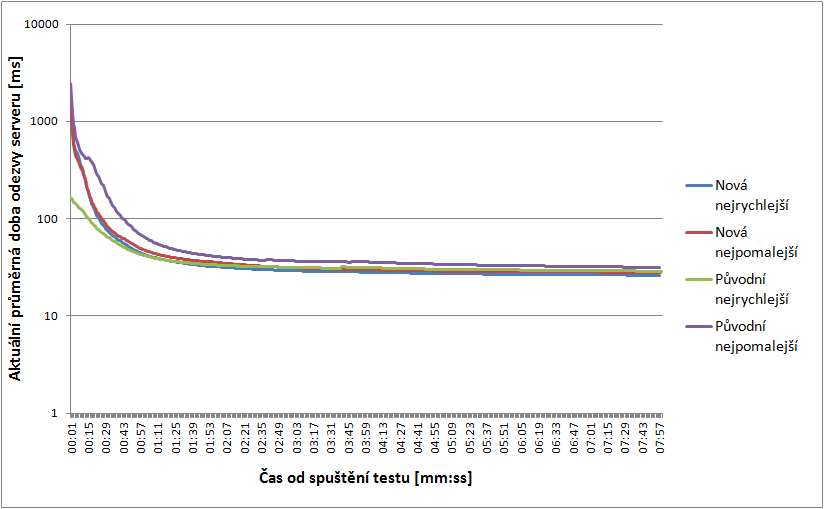
\includegraphics{img/getMainPage_cely.png}}
                    \caption{Průběh naměřených hodnot při testu získávání hlavní stránky projektu.
                        Graf zobrazuje nejlepší a nejhorší naměřené případ pro každý server.  
                        Na svislé ose je použito logaritmické měřítko.}
                    \label{imgGetMainPageCely}
                \end{center}
             \end{adjustwidth}
            \end{figure}

            \begin{figure}[h!t]
             \begin{adjustwidth}{-0.5cm}{}
                \begin{center}
                    \scalebox{0.65}{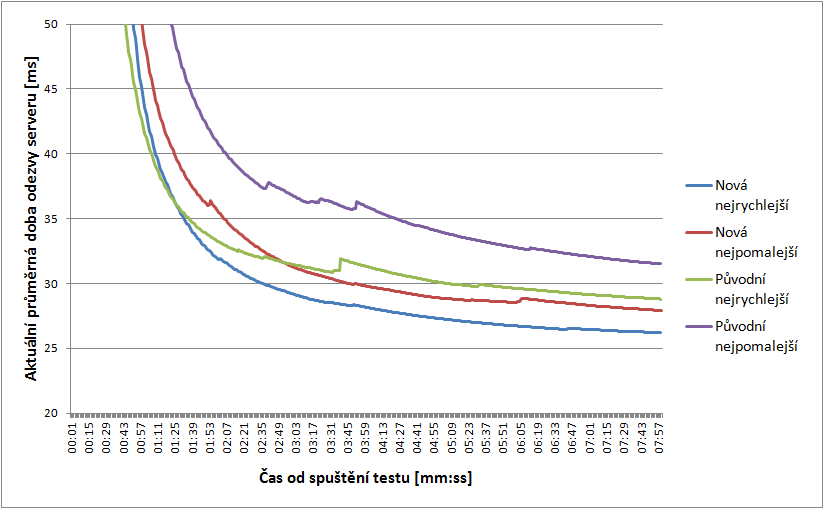
\includegraphics{img/getMainPage_cast.png}}
                    \caption{Průběh naměřených hodnot při testu získávání hlavní stránky projektu.
                        Graf zobrazuje nejlepší a nejhorší naměřené případ pro každý server.}
                    \label{imgGetMainPageCast}
                \end{center}
             \end{adjustwidth}
            \end{figure}


            \medskip
            Na počátku testů byla odezva serveru vždy vysoká, ale v průběhu docházelo k rapidnímu poklesu.
            Tento pokles a stabilní stav nastával u nové varianty serveru mírně dříve, ale ze
            směrodatné odchylky vidíme, že jeho okamžik se příliš nelišil. Hlavním
            zjištěním testu je pokles průměrné doby odezvy serveru Jenkins CI o asi 3.141 milisekund,
            což představuje zrychlení celé aplikace v průměru o \textbf{11.73\%} (dle vztahu pro výpočet \ref{eqZrychleni}).
            Z pohledu stability jednotlivých spuštění měla nová varianta Jenkins CI výrazně sníženou
            směrodatnou odchylku průměrné doby odezvy, což naznačuje konstantnější výkonnost celé aplikace.
            Tento fakt můžeme pozorovat i na grafu \ref{imgGetMainPageCast}, kde je křivka běhů nové implementace
            také stabilnější.

            Z pohledu zrychlení je důležité zdůraznit, že se jedná o zrychlení celé aplikace, takže
            zrychlení samotného servlet kontejneru bude oproti původní variantě ještě vyšší než naměřených 11.73\%.
            




        \subsection{Získání konfigurace úlohy}
            V tomto testu byly pomocí metody \texttt{GET} posílány požadavky na získání
            konfigurace jedné vytvořené úlohy na serveru (tzv. \emph{freestyle job}). 
            Testovací skript posílal požadavky pomocí \textbf{padesáti} vláken po dobu \textbf{osmi} minut.
            Pro každou variantu serveru bylo uskutečněno \textbf{10 běhů}. 

            Výsledky tohoto testu jsou zobrazeny v grafech \ref{imgGetFreestyleCely} a \ref{imgGetFreestyleCast}.
            Z naměřených dat vypočítány hodnoty aritmetického průměru a směrodatné odchylky,
            které shrnují naměřená data v experimentech (tabulka \ref{tabGetFreestyleFinal}).
            Jelikož na
            počátku testů nedocházelo vždy k poklesům hodnot okamžitě zřejmě z důvodu
            náročnosti operace, tak pro určení stabilního stavu (vzorec \ref{eqStabilni}) byla přidána
            podmínka, že průměrná hodnota doby odezvy musí být nižší než 4s.

            \begin{table}[ht]
             \catcode`\-=12
             \begin{adjustwidth}{-0.5cm}{}
             \begin{center}
              \begin{tabular}{| c || c | c || c | c |} \hline
                \multirow{3}{*}{}  &   \multicolumn{2}{c||}{\textbf{Doba odezvy}}  &  \multicolumn{2}{c|}{\textbf{Stabilní stav}}\\ \cline{2-5}
                 & \textbf{Aritmetický}  &  \textbf{Směrodatná}  &  \textbf{Aritmetický} &  \textbf{Směrodatná}\\ 
                 & \textbf{průměr} [ms]  &  \textbf{odchylka} [ms]  &  \textbf{průměr} [s]  &  \textbf{odchylka} [s]\\ \hline
                Původní verze &  1834.655 &  30.328 &  104.700 & 10.836 \\\hline
                Nová verze &  1768.139 &  20.229 &  97.300 &  5.496\\\hline
                Rozdíl &  66.516 &  10.098 &  7.400 &  5.339\\\hline  
              \end{tabular}
              \caption{Tabulka shrnující výsledky měřeného experimentu, kdy byla získávána konfigurace úlohy.}
              \label{tabGetFreestyleFinal}
             \end{center}
             \end{adjustwidth}
            \end{table}

            \begin{figure}[h!t]
             \begin{adjustwidth}{-0.5cm}{}
                \begin{center}
                    \scalebox{0.65}{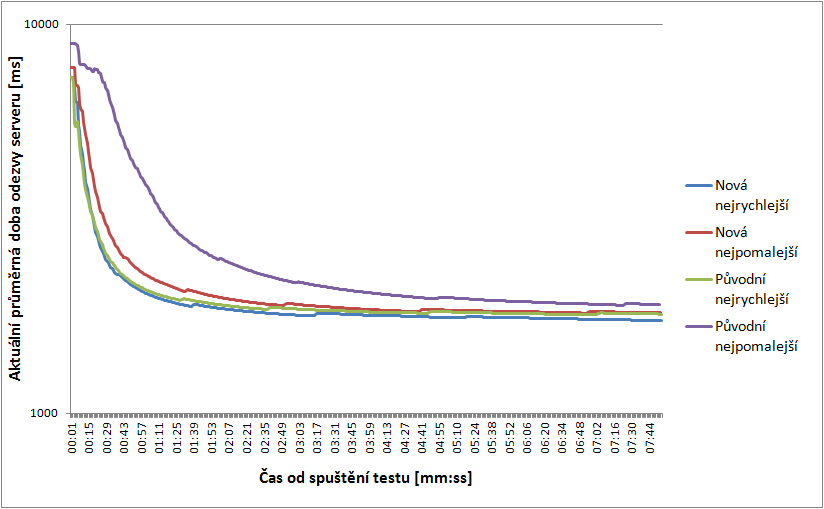
\includegraphics{img/getFreestyleJob_cely.png}}
                    \caption{Průběh naměřených hodnot při testu získávání konfigurace úlohy ze serveru.
                        Graf zobrazuje nejlepší a nejhorší naměřené případ pro každý server.  
                        Na svislé ose je použito logaritmické měřítko.}
                    \label{imgGetFreestyleCely}
                \end{center}
             \end{adjustwidth}
            \end{figure}

            \begin{figure}[h!t]
             \begin{adjustwidth}{-0.5cm}{}
                \begin{center}
                    \scalebox{0.65}{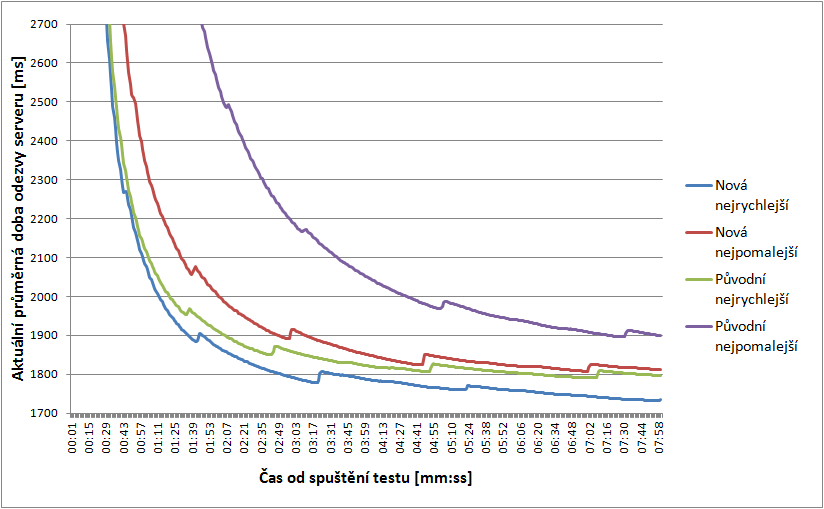
\includegraphics{img/getFreestyleJob_cast.png}}
                    \caption{Průběh naměřených hodnot při testu získávání konfigurace úlohy ze serveru.
                        Graf zobrazuje nejlepší a nejhorší naměřené případ pro každý server.}
                    \label{imgGetFreestyleCast}
                \end{center}
             \end{adjustwidth}
            \end{figure}

            V průběhu tohoto testu byl opět zaznamenán velký pokles doby odezvy na začátků experimentů.
            Z grafů vidíme, že k ustálení stavu v nové variantě docházelo v nejlepším případě v obdobné době.
            Naopak z grafův i hodnot směrodatné odchylky vidíme,
            že v nejhorší variantě byla doba ustálení u původní implementace Jenkins CI horší.

            Z pohledu naměřených hodnot průměrné doby odezvy byl zaznamenán pokles
            u nové varianty asi o 66.516 milisekund, což činí zrychlení o \textbf{3.76\%}.
            Na grafu \ref{imgGetFreestyleCast} lze vidět, že v obou variantách 
            docházelo k mírným záchvěvům v průběhu testů. Tyto stavy byly zřejmě 
            způsobeny tím, že požadavků na server docházelo velké množství
            a požadovaný úkon je výpočetně náročný. 
            Nicméně z pohledu rozptylu naměřených hodnot mezi jednotlivými
            běhy poskytovala nová varianta Jenkins CI lepší hodnoty,
            což svědčí o větší stabilitě.


        \subsection{Vytvoření nové úlohy}
            V tomto testu byly pomocí metody \texttt{POST} posílány požadavky na vytvoření
            nové úlohy na serveru (tzv. \emph{freestyle job}). Tento požadavek
            byl prováděn pomocí \emph{REST API} serveru Jenkins CI.
            Testovací skript posílal požadavky pomocí \textbf{dvou} vláken po dobu \textbf{jedné} minuty.
            Pro každou variantu serveru bylo uskutečněno \textbf{10 běhů}.

            Jelikož v průběhu testování tohoto scénáře na serveru vznikalo velmi velké množství dat v Jenkins CI (řádově stovky tisíc),
            tak musela být stanovena nižší doba testování i počet serverů, které posílají požadavky.
            Navíc před každým spuštěním byla smazána domovská složka aplikace. Pokud by smazání neproběhlo,
            tak by mohly být ovlivňovány pozdější běhy testování narůstajícím množstvím dat.

            Výsledky tohoto testu jsou zobrazeny v grafech \ref{imgCreateFreestyleCely} a \ref{imgCreateFreestyleCast}.
            V tabulce \ref{tabCreateFreestyleFinal} jsou uvedené vypočítané statistické hodnoty z
            naměřených dat.

            \begin{table}[ht]
             \catcode`\-=12
             \begin{adjustwidth}{-0.5cm}{}
             \begin{center}
              \begin{tabular}{| c || c | c || c | c |} \hline
                \multirow{3}{*}{}  &   \multicolumn{2}{c||}{\textbf{Doba odezvy}}  &  \multicolumn{2}{c|}{\textbf{Stabilní stav}}\\ \cline{2-5}
                 & \textbf{Aritmetický}  &  \textbf{Směrodatná}  &  \textbf{Aritmetický} &  \textbf{Směrodatná}\\ 
                 & \textbf{průměr} [ms]  &  \textbf{odchylka} [ms]  &  \textbf{průměr} [s]  &  \textbf{odchylka} [s]\\ \hline
                Původní verze & 19.644  &  0.381 &  10.900 & 2.914 \\\hline
                Nová verze &  19.665 &  0.282 &  15.900 & 1.814 \\\hline
                Rozdíl & $-$0.021  &  0.099 &  $-$5.000 & 1.100 \\\hline  
              \end{tabular}
              \caption{Tabulka shrnující výsledky měřeného experimentu, kdy byla vytvářena nová úloha.}
              \label{tabCreateFreestyleFinal}
             \end{center}
             \end{adjustwidth}
            \end{table}


            \begin{figure}[h!t]
             \begin{adjustwidth}{-0.5cm}{}
                \begin{center}
                    \scalebox{0.65}{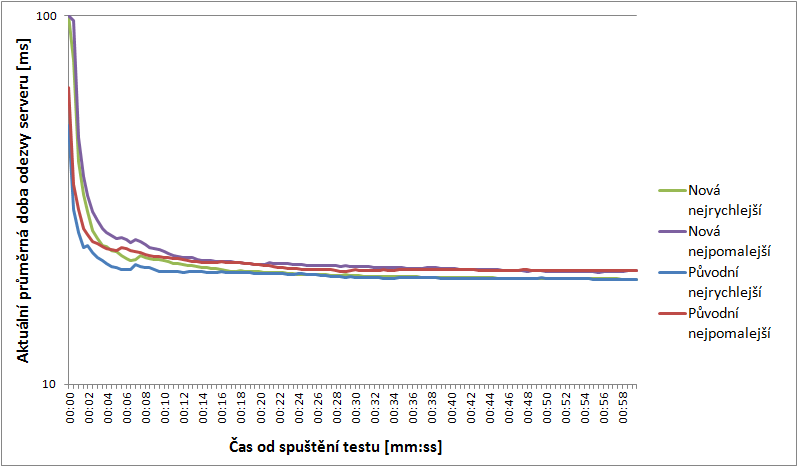
\includegraphics{img/createFreestyleJob_cely.png}}
                    \caption{Průběh naměřených hodnot při testu vytváření nové úlohy na serveru.
                        Graf zobrazuje nejlepší a nejhorší naměřené případ pro každý server.  
                        Na svislé ose je použito logaritmické měřítko.}
                    \label{imgCreateFreestyleCely}
                \end{center}
             \end{adjustwidth}
            \end{figure}

            \begin{figure}[h!t]
             \begin{adjustwidth}{-0.5cm}{}
                \begin{center}
                    \scalebox{0.65}{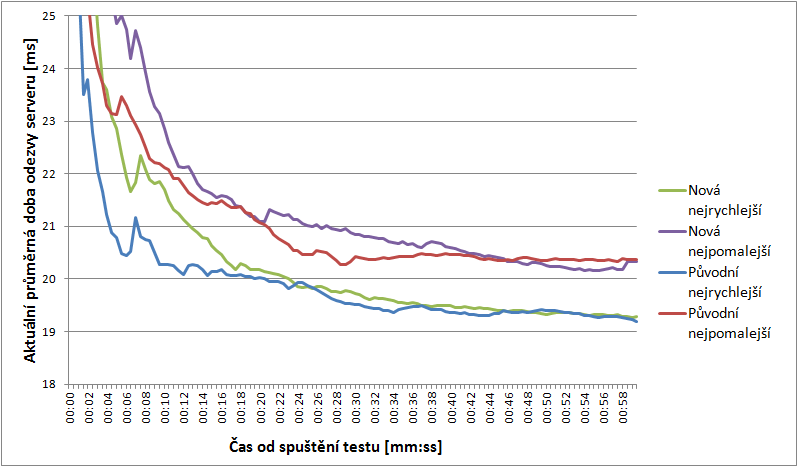
\includegraphics{img/createFreestyleJob_cast.png}}
                    \caption{Průběh naměřených hodnot při testu vytváření nové úlohy na serveru.
                        Graf zobrazuje nejlepší a nejhorší naměřené případ pro každý server.}
                    \label{imgCreateFreestyleCast}
                \end{center}
             \end{adjustwidth}
            \end{figure}

            Na počátku experimentů došlo opět k výraznému poklesu doby odezvy, ale oproti
            zbylým dvou případům se rychleji do stabilního stavu dostávala původní implementace Jenkins CI.
            Tento trend vidíme jak na grafu \ref{imgCreateFreestyleCast}, tak z průměrných
            hodnot stabilního stavu.

            V tomto testovaném případě se nepotvrdilo zrychlení nové implementace Jenkins CI,
            které bylo naměřeno v předchozích testovaných případech. Bylo naměřeno
            mírné zpomalení o -0.021 milisekund, což je vyjádřeno procenty \textbf{0.11\%}.
            Tato hodnota je velmi nízká a můžeme tedy prohlásit, že v tomto experimentu
            byly z pohledu doby odezvy obě varianty rovnocené.
            Podobnost krajních hodnoty průměrné doba odezvy je také vidět na grafu \ref{imgCreateFreestyleCast}.


    \section{Zhodnocení výsledků testování} \label{kapPerfVysledky}
        Ve třech testovacích případech byly otestovány původní implementace Jenkins CI
        a implementace s novým vestavěným servlet kontejnerem.

        V prvních dvou případech dosáhla nová implementace lepších výsledků
        výkonnosti z pohledu doby odezvy aplikace. V prvním případě zrychlení činilo téměř 12\%
        a ve druhém případě téměř 4\%. V těchto dvou případech u nové varianty
        docházelo ke stabilnějším výsledkům mezi měřeními. O trochu dříve docházelo
        také k ustálení odpovědí serveru, ale zlepšení nebylo výrazné.

        V posledním testovaném případě nebylo prokázáno zrychlení, ale mírné zpomalení o
        0.1\%. Nicméně tato hodnota je velmi nízká a lze prohlásit, že
        byly obě implementace v tomto testovaném případě stejně rychlé. 
        Z pohledu rychlosti ustálení serveru byla v tomto případě mírně lepší původní
        implementace Jenkins CI.

        \medskip
        V provedených měřeních byla tedy implementace Jenkins CI s novým
        servlet kontejnerem rychlejší než původní verze. Průměrné zrychlení
        aplikace činilo asi 5.1\% (počítáno jako aritmetický průměr ze tří hodnot zrychlení).
        Nová implementace také poskytovala stabilnější hodnoty mezi jednotlivými měřeními.

        Všechny testované činnosti ovlivňuje rychlost servlet kontejneru, ale podstatná část
        zpoždění je také ovlivněna samotnou implementací webové aplikace. Tedy je zřejmé, 
        že zrychlení samotného servlet kontejneru bylo v daných případech vyšší než
        je výsledek těchto měření.

    \section{Zhodnocení přínosu pro komunitu Jenkins CI} \label{kapPrinos}
        Cíl vytvořit servlet kontejneru založený na serveru Undertow, který bude
        funkčně kompatibiltní se stávajícím servlet kontejnerem, se podařilo
        naplnit. Tento vytvořený servlet kontejner bude v následujících dnech
        představen komunitě Jenkins CI.

        Vytvořená nová implementace servlet kontejneru  
        může pomoci nahradit zastaralou implementaci stávajícího servlet kontejneru.
        Kód původní implementace již značně degeneroval
        a je obtížně čitelný, což by tato nová verze servlet kontejneru pomohla vyřešit.

        Hlavním možným přínosem tohoto servlet kontejneru je jeho vyšší
        rychlost a výkonnost, která se v testech prokázala, ale
        určitě by bylo vhodné ještě pokračovat v dalším testování.

        Pro svůj běh Jenkins CI využívá verzi jazyka Java 6 a ještě donedávna
        udržoval kompatibilitu s verzí Java 5. Komunita
        velmi dbá na udržování zpětné kompatibility
        a nedá se tedy předpokládat,
        že v brzké době proběhne změna využívané verze jazyka.
        Problémem stávajícího servlet kontejneru je, že 
        nejnovější verze serveru Jetty odpovídá verzi Java 7.
        Z tohoto důvodu je aktuálně v Jenkins CI používána
        starší verze serveru Jetty a nebude možné přistoupit k jeho
        nahrazení verzí novější.
        Naopak server Undertow a servlet kontejner vytvořený v rámci této práce
        je kompatibilní s verzí Java 6
        a může být do budoucna dále vylepšován, což je jistá výhoda oproti stávajícímu
        stavu. 

        Pokud by se komunita rozhodla, že chce tento servlet kontejner
        začlenit do Jenkins CI, tak by bylo nutné provést ještě
        komplexnější testování nové implementace servlet kontejneru, 
        ale nebyly zjištěny žádné
        problémy které by začlenění bránily.
    


\chapter{Závěr}
    Začátek této práce se věnoval seznámení s~integračním serverem Jenkins CI,
    se servery Jetty a~Winstone, které jsou součástí jeho servlet kontejneru,
    a~se serverem Undertow, jehož integrace do Jenkins CI je hlavní
    náplní této práce. V~následující části byla analyzována architektura aplikace Jenkins CI
    a~také stav servlet kontejneru, který je v~něm integrován.

    Po seznámení se s~podmínkami pro integraci byly
    zkoumány možnosti provedení samotné integrace serveru Undertow do Jenkins CI.
    Byly zkoumány dva způsoby integrace. Jednou možností je nahrazení pouze komponenty
    Jetty, která vykonává většinu práce v~aktuálním kontejneru, zatímco druhou variantou je
    nahrazení obou součástí. 
    Po důkladném zvážení různých aspektů integrace byla 
    zvolena varianta, kdy budou nahrazeny obě komponenty současného 
    servlet kontejneru a~tudíž proběhne zcela nová implementace.



%=========================================================================




